\documentclass[fleqn,10pt,dvipsnames]{olplainarticle}
% Use option lineno for line numbers 

\title{Coursework 1, CEGE0038 Finite-Element Modelling and Numerical Methods}
\graphicspath{ {./img/} }
\author[1]{Jianer Cong}
\usepackage{tikz}
\usepackage{afterpage}
\usepackage{tcolorbox}

\affil[1]{zcesjco@ucl.ac.uk}
\keywords{Variational Principle, Galerkin's method}
\usepackage{cleveref}


\newcommand{\mycola}{Blue}
\newcommand{\mycolb}{Sepia}
\newcommand{\mycolc}{OliveGreen}

\newcommand{\cla}[1]{\textcolor{\mycola}{#1}}
\newcommand{\clb}[1]{\textcolor{\mycolb}{#1}}
\newcommand{\clc}[1]{\textcolor{\mycolc}{#1}}
\newcommand{\cld}[1]{\textcolor{gray}{#1}}

\begin{abstract}
  This report presents the answers for the following two problems:
  Problem 1 on \cpageref{sec:p1},
  Problem 2 on \cpageref{sec:p2}.
\end{abstract}

\newtcolorbox{questionbox}[1][]{
  leftrule=3mm,title={Summary of Given Conditions},sharp corners=west,#1}

\begin{document}
\maketitle
\def\MyPattern#1{My Random Prefix and #1}
\def\MySet#1#2{\expandafter\def%
  \csname\MyPattern{#1}\endcsname%
  {#2}
}
\def\MyGet#1{\csname\MyPattern{#1}\endcsname}
% \MySet{MEdl}{\textcolor{black}{45780000}}
\MySet{MEdl}{\textcolor{black}{45780000}}
\MySet{MEd}{\textcolor{black}{1.31 \ensuremath{\times 10^{8}}}}
\MySet{Asr}{\textcolor{black}{669.6}}
\MySet{n14}{\textcolor{black}{3}}
\MySet{n18}{\textcolor{black}{1}}
\MySet{As}{\textcolor{black}{716.3}}
\MySet{fcd}{\textcolor{black}{14.17}}
\MySet{Es}{\textcolor{black}{2.07 \ensuremath{\times 10^{5}}}}
\MySet{epcu}{\textcolor{black}{0.0035}}
\MySet{c}{\textcolor{black}{40}}
\MySet{qea}{\textcolor{black}{3400}}
\MySet{qeb}{\textcolor{black}{2.076 \ensuremath{\times 10^{5}}}}
\MySet{qec}{\textcolor{black}{-2.076 \ensuremath{\times 10^{7}}}}
\MySet{x}{\textcolor{black}{53.36}}
\MySet{xa}{\textcolor{black}{125}}
\MySet{eps}{\textcolor{black}{0.02929}}
\MySet{b}{\textcolor{black}{300}}
\MySet{epsp}{\textcolor{black}{0.0008765}}
\MySet{MRd}{\textcolor{black}{1.466 \ensuremath{\times 10^{8}}}}
\MySet{dh}{\textcolor{black}{4}}
\MySet{d}{\textcolor{black}{500}}
\MySet{Asw}{\textcolor{black}{25.13}}
\MySet{VEd}{\textcolor{black}{87.8}}
\MySet{fyd}{\textcolor{black}{434.8}}
\MySet{rho}{\textcolor{black}{0.0048}}
\MySet{sreq}{\textcolor{black}{56.01}}
\MySet{sact}{\textcolor{black}{50}}
\MySet{VRdsAct}{\textcolor{black}{98.35}}
\MySet{smax}{\textcolor{black}{96}}
\MySet{sactn}{\textcolor{black}{100}}
\MySet{VRdsActn}{\textcolor{black}{122.9}}
\MySet{smaxn}{\textcolor{black}{375}}
\MySet{sreqn}{\textcolor{black}{140}}
\MySet{b2.MEdl}{\textcolor{black}{45780000}}
\MySet{b2.MEd}{\textcolor{black}{1.945 \ensuremath{\times 10^{8}}}}
\MySet{b2.Asr}{\textcolor{black}{994.1}}
\MySet{b2.n14}{\textcolor{black}{0}}
\MySet{b2.n18}{\textcolor{black}{4}}
\MySet{b2.As}{\textcolor{black}{1018}}
\MySet{b2.fcd}{\textcolor{black}{14.17}}
\MySet{b2.Es}{\textcolor{black}{2.07 \ensuremath{\times 10^{5}}}}
\MySet{b2.epcu}{\textcolor{black}{0.0035}}
\MySet{b2.c}{\textcolor{black}{40}}
\MySet{b2.qea}{\textcolor{black}{3400}}
\MySet{b2.qeb}{\textcolor{black}{2.95 \ensuremath{\times 10^{5}}}}
\MySet{b2.qec}{\textcolor{black}{-2.95 \ensuremath{\times 10^{7}}}}
\MySet{b2.x}{\textcolor{black}{59.37}}
\MySet{b2.xa}{\textcolor{black}{125}}
\MySet{b2.eps}{\textcolor{black}{0.02597}}
\MySet{b2.b}{\textcolor{black}{300}}
\MySet{b2.epsp}{\textcolor{black}{0.001142}}
\MySet{b2.MRd}{\textcolor{black}{2.069 \ensuremath{\times 10^{8}}}}
\MySet{b2.dh}{\textcolor{black}{6}}
\MySet{b2.d}{\textcolor{black}{500}}
\MySet{b2.Asw}{\textcolor{black}{56.55}}
\MySet{b2.VEd}{\textcolor{black}{124.4}}
\MySet{b2.fyd}{\textcolor{black}{434.8}}
\MySet{b2.rho}{\textcolor{black}{0.0068}}
\MySet{b2.sreq}{\textcolor{black}{88.94}}
\MySet{b2.sact}{\textcolor{black}{50}}
\MySet{b2.VRdsAct}{\textcolor{black}{221.3}}
\MySet{b2.smax}{\textcolor{black}{112}}
\MySet{b2.sactn}{\textcolor{black}{200}}
\MySet{b2.VRdsActn}{\textcolor{black}{138.3}}
\MySet{b2.smaxn}{\textcolor{black}{375}}
\MySet{b2.sreqn}{\textcolor{black}{222}}
\MySet{cl.N}{\textcolor{black}{7.466 \ensuremath{\times 10^{5}}}}
\MySet{cl.b}{\textcolor{black}{400}}
\MySet{cl.h}{\textcolor{black}{600}}
\MySet{cl.vd}{\textcolor{black}{0.2196}}
\MySet{cl.rho}{\textcolor{black}{0.01}}
\MySet{cl.Asmin}{\textcolor{black}{2400}}
\MySet{cl.Asa}{\textcolor{black}{2545}}
\MySet{cl.barn}{\textcolor{black}{10}}
\MySet{cl.bard}{\textcolor{black}{18}}
\MySet{cl.MRd.bx}{\textcolor{black}{146}}
\MySet{cl.MRd.by}{\textcolor{black}{123}}
\MySet{cl.MRd.cx1}{\textcolor{black}{225}}
\MySet{cl.MRd.cx2}{\textcolor{black}{220}}
\MySet{cl.MRd.cy1}{\textcolor{black}{180}}
\MySet{cl.MRd.cy2}{\textcolor{black}{178}}
\MySet{cl.SMRd.bx}{\textcolor{black}{379.6}}
\MySet{cl.SMRd.by}{\textcolor{black}{319.8}}
\MySet{cl.SMRd.cx}{\textcolor{black}{445}}
\MySet{cl.SMRd.cy}{\textcolor{black}{358}}
\MySet{cl.N.c1}{\textcolor{black}{716}}
\MySet{cl.N.c2}{\textcolor{black}{516.2}}
\MySet{cl.shr.MRdc}{\textcolor{black}{225}}
\MySet{cl.shr.Lclr}{\textcolor{black}{2800}}
\MySet{cl.shr.VEdcol}{\textcolor{black}{176.8}}
\MySet{cl.shr.dh}{\textcolor{black}{4}}
\MySet{cl.shr.d}{\textcolor{black}{600}}
\MySet{cl.shr.Asw}{\textcolor{black}{62.83}}
\MySet{cl.shr.VEd}{\textcolor{black}{176.8}}
\MySet{cl.shr.fyd}{\textcolor{black}{434.8}}
\MySet{cl.shr.rho}{\textcolor{black}{0.0005236}}
\MySet{cl.shr.sreq}{\textcolor{black}{83.44}}
\MySet{cl.shr.sact}{\textcolor{black}{50}}
\MySet{cl.shr.VRdsAct}{\textcolor{black}{295}}
\MySet{cl.shr.smax}{\textcolor{black}{112}}
\MySet{cl.shr.sactn}{\textcolor{black}{200}}
\MySet{cl.shr.VRdsActn}{\textcolor{black}{184.4}}
\MySet{cl.shr.smaxn}{\textcolor{black}{450}}
\MySet{cl.shr.sreqn}{\textcolor{black}{208.6}}
\MySet{cl.bi}{\textcolor{black}{320}}
\MySet{cl.bi2}{\textcolor{black}{175}}
\MySet{cl.b0}{\textcolor{black}{328}}
\MySet{cl.h0}{\textcolor{black}{528}}
\MySet{cl.s}{\textcolor{black}{50}}
\MySet{cl.aln}{\textcolor{black}{0.6439}}
\MySet{cl.als}{\textcolor{black}{0.883}}
\MySet{cl.phi}{\textcolor{black}{4}}
\MySet{cl.omwd}{\textcolor{black}{0.09883}}
\MySet{cl.fyd}{\textcolor{black}{434.8}}
\MySet{cl.fcd}{\textcolor{black}{14.17}}
\MySet{cl.al}{\textcolor{black}{0.5685}}
\MySet{cl.alom}{\textcolor{black}{0.05619}}

\section*{Qestion 1: convective heat flow in a tapered fin}\label{sec:p1}
\newcommand{\lhs}{%
  \ensuremath{-(x T')' + \alpha (T - T_{_{\infty}})}
}

\begin{questionbox}
  The temperature distribution $T$ is governed by

  \begin{align}
    \lhs & = 0,
    & (0 \leq x \leq L) \label{eq:base}
  \end{align}
  Where BCs are
  \begin{align}
    {[xT']}_{x=0} &= 0 \label{eq:bc1}\\
    T(L) &= T_0 \label{eq:bc2}
  \end{align}
  And the constants are $L = 4, T_0 = 250, T_{\infty} = 75, \alpha = 0.4168$.
\end{questionbox}

\subsection*{Answer}\label{sec:q1}

\subsubsection*{Applying variational principle}
Applying variational principle, we put the LHS of \cref{eq:base} into the
integral with $\delta T$
\renewcommand{\i}[1]{\ensuremath{\int_0^L #1 dx}}
\begin{align}
  \i{[\lhs] \delta T} &=0 \notag\\
                      &= \cla{-\i{(xT')' \delta T}}
                        +\clb{\i{\alpha T \delta T}}
                        -\clc{\i{\alpha T_{\infty} \delta T}} \label{eq:base2}\\
                      &:= \cla{[1]} + \clb{[2]} + \clc{[3]} \notag
\end{align}

\subsubsection*{Term $\cla{[1]}$}
For $\cla{[1]}$, we integrate by part:
\def\bdr{\cld{\ensuremath{{[xT' \delta T]}_0^L}}}
\def\Bdr{\cld{\ensuremath{{[xT' T]}_0^L}}} %bdr without $\delta$
\begin{align*}
  \cla{[1]} &= -(\bdr - \i{\delta T' x T'}) \\
            &= -(\cdots - \i{x \delta(\frac{1}{2} T'^2) }) \\
            &= -(\cdots - \i{\delta(x\frac{1}{2} T'^2)})
\end{align*}
The term \bdr{} will form the \emph{boundary vector}.

Therefore, $\cla{[1]}$ becomes

\def\aai{x\frac{1}{2} T'^2}
\def\aa{\delta(\aai)}
\begin{align}
  \cla{[1] = \i{\aa}} - \bdr \label{eq:1}
\end{align}

\def\b{\ensuremath{\clb{[2]}}}
\def\c{\ensuremath{\clc{[3]}}}
\subsubsection*{Terms \b and \c}
For \b and \c:
\def\bbi{\frac{\alpha}{2}T^2}
\def\bb{\delta(\bbi)}
\def\cci{\alpha T_{\infty} T}
\def\cc{-\delta(\cci)}
\begin{align}
  \b &= \clb{\i{\alpha \delta (\frac23 T^2)} = \i{\bb}}\label{eq:2}\\
  \c &= \clc{\i{\cc}} \label{eq:3}
\end{align}

\subsubsection*{Putting them back}
Substituting \cref{eq:1,eq:2,eq:3} back to \cref{eq:base2} gives

\newcommand{\thethree}[5]{\cla{#1} #4 \clb{#2} #5 \clc{#3}}
\begin{align}
  % \cla{[1]} + \clb{[2]} + \clc{[3]}
  \thethree{[1]}{[2]}{[3]}{+}{+}
  % &= \i{\aa} + \i{\bb} + \i{\cc} \notag\\
    &= \thethree{\i{\aa}}{\i{\bb}}{\i{\cc}}{+}{+}  - \bdr \notag\\
    % &= \i{\aa + \bb \cc} \notag\\
    &= \i{\thethree{\aa}{\bb}{\cc}{+}{}}  -\bdr \notag\\
    % &=\delta\i{\aai + \bbi - \cci} \notag\\
    &= \delta \left(\i{\thethree{\aai}{\bbi}{\cci}{+}{-}} - \Bdr \right)
      \label{eq:4}
\end{align}
Now \cref{eq:4} gives us
\begin{align}
  \mbox{The variational principle problem} =
  \begin{cases}
    I[T] &:= \i{\thethree{\aai}{\bbi}{\cci}{+}{-} - \Bdr} \\
    \delta T &= 0
  \end{cases} \label{eq:var}
\end{align}

\subsubsection*{Substitute model function}
According to Galerkin's method, if we have n nodes, then we take the following
model function $T_{t}(x)$:\footnote{Here we use the \emph{Einstein notation},
  which is the convention that says ``Repeating indexes imply summation''. For
  example, $a_i b_i = \sum_i a_i b_i$ and $K_{ij}v_j = \sum_j K_{ij} v{j}$.}

\begin{align}
  T_t(x) &:= N_i T_i & i = (1 ,\ldots , n )\label{eq:testfun}
\end{align}
Where $N_i = N_i(x)$ is the shape function for node $i$, and $T_i$ is the
temperature on node $i$.

Substituting $T = T_t$ in \cref{eq:testfun} back into \cref{eq:var} gives
\def\x{\ensuremath{\alpha T_{\infty} N_i T_i}}
\newcommand{\eBdri}[1]{\ensuremath{{[xT']}_{#1}}}  %an elaborate term
\newcommand\eBdr[1]{\ensuremath{\eBdri{#1} T(#1)}} % End of boundary
\newcommand{\twoBdr}{\ensuremath{
    \left(\cld{\eBdr{L} - \eBdr{0}}\right)
  }}
\begin{align}
  I[T_i] &:= \i{\thethree{\frac{x}{2} {(N_i T_i)'}^2}
           {\frac{\alpha}{2} {(N_i T_i)}^2}{\x}{+}{-}
           }- \twoBdr
           \notag\\
         &=\thethree{\i{T_i \frac{x}{2} N_i' N_j' T_j}}
           {\i{\frac{\alpha}{2} T_i N_i N_j T_j}}
           {\i{\x}}{+}{-} - \cld{\dotsb}
           \notag\\
         &= \thethree{T_i \i{ \frac{x}{2} N_i' N_j' } T_j}
           {T_i \i{\frac{\alpha}{2} N_i N_j} T_j}
           {\alpha T_{\infty} \i{N_i} T_i}{+}{-} - \cld{\dotsb}
           \label{eq:6}
\end{align}
Now, define
\begin{align*}
  \cla{K_{ij}} & := \cla{\i{xN_i' N_j'}}     \\
  \clb{L_{ij}} & := \clb{\i{\alpha N_i N_j}} \\
  \clc{b_i}    & := \clc{\alpha T_{\infty} \i{N_i}}  \\
  \cld{c} &:= \twoBdr{} \\
  M_{ij} & := L_{ij} + K_{ij}
\end{align*}
Then \cref{eq:6} becomes
\def\c{\cld{c}}
\begin{align*}
  I[T_i] &= \thethree{\frac{1}{2} T_i K_{ij} T_j}
           {\frac{1}{2} T_i K_{ij} T_j}{b_i T_i}{+}{-} - \c \\
         &= \frac{1}{2} T_i M_{ij} T_j - b_i T_i  - \c
\end{align*}

\def\T{\mathbf{T}}
\def\M{\mathbf{M}}
\def\b{\mathbf{b}}
\def\c{\mathbf{c}}

Setting the derivatives with respect to $\T := [T_1, \dotsc , T_{n}]$ equal to
zero gives:
\newcommand{\pFrac}[2]{\ensuremath{\frac{\partial #1}{\partial #2}}}
\newcommand{\pcTk}{\ensuremath{\cld{\pFrac{c}{T_k}}}}
\begin{align}
 \pFrac{I[T]}{T_k} &= \frac{1}{2}[T_i M_{ik} + M_{kj}T_j] - b_k - \pcTk
                                       = M_{k,j}T_j - b_k - \pcTk \notag\\
  \frac{\partial I[T]}{\partial \T }
                   &= \M\T - \b - \c= \mathbf{0} \notag\\
  \M \T &= \b + \c \label{eq:mtb}
\end{align}
Where
\newcommand{\tsps}[1]{\ensuremath{{#1}^{\text{T}}}}
\newenvironment{tbmatrix}{\begin{bmatrix}}{\end{bmatrix}^{\text{T}}}
\begin{align*}
  \M &=
       \begin{bmatrix}
         M_{11} & \cdots& M_{1n}\\
         \vdots& \ddots &\\
         M_{n1}&& M_{nn} \\
       \end{bmatrix} &
                       \b &=
                            % \tsps{\begin{bmatrix}
                            %   b_1 & \dotsc & b_n
                            % \end{bmatrix}} \\
                            \begin{tbmatrix}
                              b_1 & \dotsc & b_n
                            \end{tbmatrix} \\
  \c &=\begin{tbmatrix}
    -\eBdri{0} & 0 & \dotsc & 0 & \eBdri{L}
       \end{tbmatrix}
\end{align*}

\subsubsection*{Calculate $\c$}
Since we use a three-node mesh as shown on \cref{fig:shpfuncs}. $\c$ is
\begin{align}
  \c &=\begin{tbmatrix}
    -\eBdri{0}&0&0&0& \eBdri{L}
  \end{tbmatrix}
                      \notag\\
  \intertext{Applying the boundary condition \cref{eq:bc1} gives}
  \c &=\begin{tbmatrix}
    0&0&0&0& \eBdri{L}
  \end{tbmatrix} \label{eq:bigc}
\end{align}
And the term $\eBdri{L}$ is another unknown that the question asked for.
\begin{figure}
  \centering
  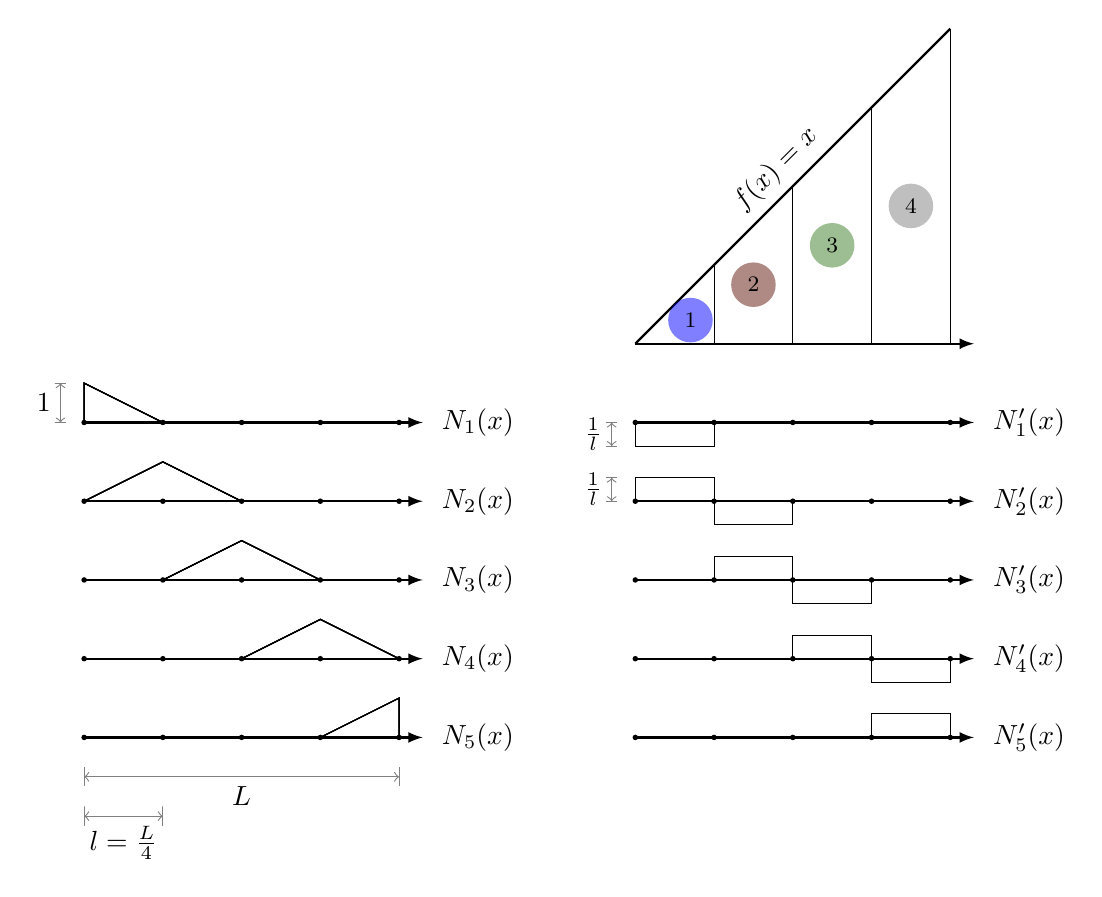
\begin{tikzpicture}[x=1cm,y=1cm]
  \begin{scope}
    % \draw[style=help lines,step=1cm] (0,-1) grid (11,5);

    \foreach \y in {0,1,2,3,4}{%
      \foreach \x in {0,7}{%
        \draw[-latex,thick] (\x,\y) -- +(4.3,0);
        \foreach \z in {0,1,2,3,4}{
          \fill[black] (\x + \z, \y) circle (1pt);
        }
      }



      \newcommand{\myh}{0.5}
      \draw (0,4) -- ++(0,\myh) -- ++(1,-\myh);
      \draw (3,0) -- ++(1,\myh) -- ++(0,-\myh);
      \foreach \i in {0,1,2}{
        \draw (\i, 3 - \i) -- ++(1,\myh) -- ++(1,-\myh);
      }
    }

    \foreach \i in {0,1,2,3}{
      \foreach \j in {0,0.7}{
        \draw (7 + \i, 3 - \i + \j) rectangle +(1,0.3);
      }
    }
    \foreach \y in {1,2,3,4,5}{
      % Label each diagram
      \node at (5, 5 - \y) {$N_{\y}(x)$};
      \node at (5 + 7, 5 - \y) {$N_{\y}'(x)$};
    }

  \end{scope}

  \newdimen\h
  \h=3.5pt

  % Draw the two dimensions
  \begin{scope}[draw=black!50]
    \foreach \i / \j / \l in {0.5 / 4 / L, 1 / 1 / l=\frac{L}{4}}{
      \draw[thin,<->] (0,-\i) to node[anchor=north] {$\l$} +(\j,0);
      \draw (0,-\i) -- +(0,\h) -- +(0, -\h)
      (\j,-\i) -- +(0,\h) -- +(0, -\h);
    }

    \h=2pt
    \newcommand{\mydimy}[4]{%
      \draw[thin,<->] (#1,#2) to node[left] {#4} +(0,#3);
      \draw (#1,#2) -- +(-\h,0) -- +(\h,0)
      (#1,#2 + #3) --  +(-\h,0) -- +(\h,0);
    }
    % \draw[thin,<->] (-0.3,4) to node[left] {1} +(0,0.5);
    % \draw (-0.3,4) -- +(-\h,0) -- +(\h,0)
    % (-0.3,4 + 0.5) --  +(-\h,0) -- +(\h,0);
    \mydimy{-0.3}{4}{0.5}{1}
    \mydimy{7-0.3}{3}{0.3}{$\frac{1}{l}$}
    \mydimy{7-0.3}{3.7}{0.3}{$\frac{1}{l}$}
  \end{scope}

  \begin{scope}[xshift=7cm,yshift=5cm]
    \draw[-latex,thick] (0,0) -- +(4.3,0);
    \draw[thick] (0,0) to node[sloped,above]{$f(x)=x$} (4,4);
    \foreach \x in {1,2,3,4}{
      \draw (\x,0) -- (\x,\x);
    }

    \newcommand{\mynode}[3][(0,0)]{
      \node[shape=circle, fill=#3,
      fill opacity=0.5,text opacity=1,font=\footnotesize, shift={#1}] {#2};
      % \node[shape=circle, fill=gray,
      % fill opacity=0.5,text opacity=1,font=\footnotesize, shift={(1cm,1cm)}] {2};
    }
    % \foreach \i/\j/\c in {0.5/1/\mycola,1.3/2/\mycolb,2.3/3/\mycolc,3.3/4/gray}{
    %   \mynode[(\i + 0.2, \i -0.2)]{\j}{\c}
    % }
    \mynode[(0.7, 0.3)]{1}{\mycola}
    \mynode[(1.5,0.75)]{2}{\mycolb}
    \mynode[(2.5,1.25)]{3}{\mycolc}
    \mynode[(3.5,1.75)]{4}{gray}
    % \mynode[(0.5 + 0.2, 0.5 -0.2)]{2}{\mycolb}
    % \mynode[(0.5 + 0.2, 0.5 -0.2)]{3}{\mycolc}
  \end{scope}

\end{tikzpicture}
  \caption{Shape functions and their derivative}\label{fig:shpfuncs}
\end{figure}
\subsubsection*{Calculate $K_{ij}$}
The shape functions and their derivatives are presented on \cref{fig:shpfuncs}.
We first calculate the diagonal entries:


\newcommand{\mynode}[3][]{
  \begin{tikzpicture}
    \def\h{17pt}
    \useasboundingbox (0,0) rectangle (\h,\h);
    \node[shape=circle, fill=#3,
    fill opacity=0.5,text opacity=1,font=\footnotesize, shift={(8.5pt,3pt)}] {#2};
  \end{tikzpicture}
}

\newcommand{\na}{\mynode{1}{\mycola}}
\newcommand{\nb}{\mynode{2}{\mycolb}}
\newcommand{\nc}{\mynode{3}{\mycolc}}
\newcommand{\nd}{\mynode{4}{gray}}

\begin{align}
  K_{11} &= \i{x N_0' N_0'}
           = [\text{area of \na on \cref{fig:shpfuncs}}]
           \times {[\text{the slope of shape function}]}^2
           :=  \na \times s \label{eq:k11}\\
  K_{22} &= \i{xN_1' N_1'} = [\text{area of \na{} $+$ \nb{}}]
           \times {[\text{the slope of shape function}]}^2
           := (\na{} + \nb{}) \times s \label{eq:k22}\\
  \intertext{Similarly}
  K_{33} & = (\nb{} + \nc{}) \times s \label{eq:k33}\\
  K_{44} & = (\nc{} + \nd{}) \times s \label{eq:k44}\\
  K_{55} &= (\nd{}) \times s \label{eq:k55}
\end{align}
Note that in \cref{eq:k11,eq:k22,eq:k33,eq:k44,eq:k55}, they are all multiplied by the same value $s = \frac{1}{l^2}$, even if
the slope is sometimes positive and sometimes negative. This is because, when
they are squared, they are always positive.

Now the areas can be calculated as follows:
\begin{align}
  \na &= \frac{l^2}{2} \label{eq:na}\\
  \nb &= l^2 + \na = \frac{3}{2}l^2 \label{eq:nb}\\
  \nc &= l^2 + \nb = \frac{5}{2}l^2 \label{eq:nc}\\
  \nd &= l^2 + \nc = \frac{7}{2}l^2 \label{eq:nd}
\end{align}
Substituting \cref{eq:na,eq:nb,eq:nc,eq:nd} back into
\cref{eq:k11,eq:k22,eq:k33,eq:k44,eq:k55} gives
\begin{align}
  K_{11} &=  \na \times s =
           \frac{l^2}{2} \times \frac{1}{l^2}
           = \frac{1}{2}\label{eq:nk11}\\
  K_{22} &= (\na{} + \nb{}) \times s =
           (\frac{l^2}{2} + \frac{3}{2}l^2) \frac{1}{l^2} =
           \frac{1}{2} + \frac{3}{2} = \frac{4}{2}
           \label{eq:nk22}\\
  K_{33} & = (\nb{} + \nc{}) \times s
           (\frac{3}{2}l^2 + \frac{5}{2}l^2) \frac{1}{l^2} =
           \frac{3}{2} + \frac{5}{2} = \frac{8}{2}
           \label{eq:nk33}\\
  K_{44} & = (\nc{} + \nd{}) \times s =
           \frac{5}{2} + \frac{7}{2} = \frac{23}{2}
           \label{eq:nk44}\\
  K_{55} &= \nd{} \times s = \frac{7}{2}
           \label{eq:nk55}
\end{align}

Now for the off-diagonal entries, because
\def\K{\ensuremath{\mathbf{K}}}
\begin{enumerate}
\item $\K$ is symmetrical ($K_{ij} = K_{ji}$)
\item the product of two node's shape functions is zero if the nodes are not
  next to each other
\end{enumerate}
the only entries that we need to calculate are the following
\begin{align}
  K_{12} &
           = [\text{area of \na{} on \cref{fig:shpfuncs}}]
           \times - {[\text{the slope of shape function}]}^2
           = \na{} \times (-s)  = -\frac{1}{2}\label{eq:nk12}\\
  K_{23} &= \nb{} \times (-s) = -\frac{3}{2}\label{eq:nk23}\\
  K_{34} &= \nc{} \times (-s) = -\frac{5}{2}\label{eq:nk34}\\
  K_{45} &= \nd{} \times (-s) = -\frac{7}{2}\label{eq:nk45}
\end{align}

Combining
\cref{eq:nk12,eq:nk23,eq:nk34,eq:nk45,eq:nk11,eq:nk22,eq:nk33,eq:nk44,eq:nk55}
gives the matrix $\K$
\def\matK{\ensuremath{\frac{1}{2}
    \begin{bmatrix}
      1 & -1 &&&\\
      -1 &4&-3&&\\
      & -3 &8&-5&\\
      &&-5&12&-7\\
      &&&-7&7
    \end{bmatrix}
  }}
\begin{align}
  \K &=
               \begin{bmatrix}
                 K_{11} & K_{12} &&&\\
                 K_{12} & K_{22} &K_{23}&&\\
                 & K_{23} &K_{33}&K_{34}&\\
                 &&K_{34}&K_{44}&K_{45}\\
                 &&&K_{45}&K_{55}
               \end{bmatrix} = \matK{} \label{eq:bigK}
\end{align}
In \cref{eq:bigK}, empty entry implies zero.

\subsubsection*{Calculate $L_{ij}$}
\def\L{\ensuremath{\mathbf{L}}}
Before we calculate \L, we calculate two \emph{convolution integrals}
% Triangle A
\newcommand{\Ta}{
  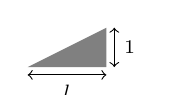
\begin{tikzpicture}
    \tikzstyle{every node}=[font=\scriptsize]
    \def\w{1cm}
    \def\h{0.5cm}
    \useasboundingbox (0,0) rectangle (\w + 15pt, \h);
    \fill[gray] (0,0) -- (\w,\h) -- (\w,0) -- cycle;
    % Draw the two dimensions
    % \def\h{3.5pt}
    \def\i{0.1cm}
    \draw[thin,<->] (0,-\i) to node[below] {$l$} +(\w,0);
    \draw[thin,<->] (\w + \i,0) to node[right] {1} +(0,\h);
  \end{tikzpicture}
}
% Triangle B
\newcommand{\Tb}{
  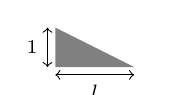
\begin{tikzpicture}
    \tikzstyle{every node}=[font=\scriptsize]
    \def\w{1cm}
    \def\h{0.5cm}
    \useasboundingbox (-10pt,0) rectangle (\w + 5pt, \h);
    \fill[gray] (0,0) -- (0,\h) -- (\w,0) -- cycle;
    \def\i{0.1cm}
    \draw[thin,<->] (0,-\i) to node[below] {$l$} +(\w,0);
    \draw[thin,<->] (-\i,0) to node[left] {1} +(0,\h);
  \end{tikzpicture}
}

\newcommand{\il}[1]{\ensuremath{\int_0^l #1 dx}}
\newcommand{\brkIt}[1]{\ensuremath{\left[#1\right]}}
\newcommand{\brkItl}[1]{\ensuremath{{\brkIt{#1}}_0^l}}
\newcommand{\prnIt}[1]{\ensuremath{\left( #1 \right)}}
\def\xl{\ensuremath{{\left( \frac{x}{l} \right)}^2}}
% \def\a{\cla{a}}
% \def\b{\clb{b}}
\def\a{\tcbox[on line,size=small,colback=\mycola!20,colframe=\mycola]{a}}
\def\b{\tcbox[on line,size=small,colback=\mycolb!20,colframe=\mycolb]{b}}
\def\anum{\ensuremath{\alpha\frac{l}{3}}}
\def\bnum{\ensuremath{\alpha\frac{l^2}{2} - \anum }}
\def\bnumb{\ensuremath{\alpha\frac{l}{6}(3l-2)}}
\begin{align}
  \a &:= \alpha \il{\Ta \Ta} = \alpha  \il{\xl{}} \notag\\
  &= \alpha \frac{1}{l^2} \brkItl{\frac{1}{3}x^3}
  = \frac{l^3}{3l^2} = \anum \\[\baselineskip]
  \b &:= \alpha \il{\Ta \Tb } = \alpha  \il{\frac{x}{l} (l - \frac{x}{l})} \notag\\
    &= \alpha\il{x} - \alpha \il{\xl{}}
      = \alpha\brkItl{\frac{x^2}{2}} - \a \notag\\
  &= \bnum =  \bnumb
\end{align}
Now, because $L_{ij} := \alpha \i{N_i N_j}$, from \cref{fig:shpfuncs} we see
that
\begin{align}
  L_{11} &= L_{55} = \a  = \anum \label{eq:l1}\\
  L_{22} &= L_{33} = L_{44} = 2 \times \a = \alpha\frac{2l}{3} \label{eq:l2}\\
  L_{12} &= L_{23} = L_{34} = L_{45} = \b = \bnumb \label{eq:l3}
\end{align}
\def\L{\ensuremath{\mathbf{L}}}
Since \L \ has the same properties as \K \
(i.e.,being symmetrical, non-neibour entries have value of 0).
Combining \cref{eq:l1,eq:l2,eq:l3} gives the matrix \L
\def\x{3l-2}
\begin{align}
  \mathbf{L} &=
               \begin{bmatrix}
                 L_{11} & L_{12} &&&\\
                 L_{12} & L_{22} &L_{23}&&\\
                 & L_{23} &L_{33}&L_{34}&\\
                 &&L_{34}&L_{44}&L_{45}\\
                 &&&L_{45}&L_{55}
               \end{bmatrix}
                            =
                            \frac{\alpha l}{6}
                            \begin{bmatrix}
                              2& c &&&\\
                              c &4&c&&\\
                              & c &4&c&\\
                              &&c&4&c\\
                              &&&c&2
                            \end{bmatrix} \label{eq:bigL}\\
  c &:= \x \notag
\end{align}
In \cref{eq:bigL}, empty entry implies zero.

\subsubsection*{Calculate $b_i$}
\def\b{\ensuremath{\mathbf{b}}}
\def\matb{\ensuremath{
    \begin{bmatrix}
      1 \\ 2  \\ 2 \\ 2 \\ 1
    \end{bmatrix}
  }}
The last array needed for \cref{eq:mtb} is \b \ where
\def\aTi{\ensuremath{\alpha T_{\infty}}}
\def\A{\tcbox[on line,size=small,colback=\mycolc!20,colframe=\mycolc]{A}}
\def\alT{\ensuremath{\alpha T_{\infty}}}
\begin{align}
  \clc{b_i} :&= \clc{\aTi \i{N_i}} \notag\\
             &= \aTi  \times [\text{The area under shape function \ } N_i(x)] \notag\\
  \intertext{Therefore}
  \b &= \A \matb
       \quad \text{where \ } \A = \alT \times \left[
       \text{area of \Ta}  = \frac{l}{2} \right] \label{eq:bigb}
\end{align}

\subsubsection*{Back to the system}
Now, substituting \cref{eq:bigc,eq:bigK,eq:bigL,eq:bigb} back into \cref{eq:mtb} gives
the system
\def\M{\ensuremath{\mathbf{M}}}
\def\matM{\ensuremath{
    \begin{bmatrix}
      \frac{\alpha}{3} + \frac{1}{2} & \frac{\alpha}{6} - \frac{1}{2} &&&\\
      \frac{\alpha}{6} - \frac{1}{2} & \frac{2 \alpha}{3} + 2& \frac{\alpha}{6} - \frac{3}{2} &&\\
       &\frac{\alpha}{6} - \frac{3}{2}&\frac{2 \alpha}{3} + 4& \frac{\alpha}{6} - \frac{5}{2} &\\
       && \frac{\alpha}{6} - \frac{5}{2}&\frac{2 \alpha}{3} + 6& \frac{\alpha}{6} - \frac{7}{2}\\
       &&& \frac{\alpha}{6} - \frac{7}{2}&\frac{\alpha}{3} + \frac{7}{2}
      \end{bmatrix}
  }}
\def\matMmoved{\ensuremath{
    \begin{bmatrix}
      \frac{\alpha}{3} + \frac{1}{2} & \frac{\alpha}{6} - \frac{1}{2} &&\\
      \frac{\alpha}{6} - \frac{1}{2} & \frac{2 \alpha}{3} + 2& \frac{\alpha}{6} - \frac{3}{2} &\\
      &\frac{\alpha}{6} - \frac{3}{2}&\frac{2 \alpha}{3} + 4& \frac{\alpha}{6} - \frac{5}{2} \\
      && \frac{\alpha}{6} - \frac{5}{2}&\frac{2 \alpha}{3} + 6\\
      &&& \frac{\alpha}{6} - \frac{7}{2}
    \end{bmatrix}
  }
}

\begin{align}
  \M &= \L + \K =
  \frac{\alpha l}{6}
  \begin{bmatrix}
    2& c &&&\\
    c &4&c&&\\
    & c &4&c&\\
    &&c&4&c\\
    &&&c&2
  \end{bmatrix} + \matK \notag\\
  c &= \x \notag\\
  \b &=\alT \frac{l}{2}\begin{bmatrix}1&2&2&2&1\end{bmatrix}^{\text{T}} \notag\\
  \intertext{Substituting $l = \frac{4}{4} = 1$
  gives}
  c &= 1 \notag\\
  \M &=
       \frac{\alpha}{6}
       \begin{bmatrix}
         2& 1 &&&\\
         1 &4&1&&\\
         & 1 &4&1&\\
         &&1&4&1\\
         &&&1&2
       \end{bmatrix} + \matK \notag\\
     &=\MyGet{M} \label{eq:bigM}\\
  \b &=\alT \frac{1}{2}\begin{bmatrix}1&2&2&2&1\end{bmatrix}^{\text{T}} \notag \\
\end{align}
Therefore the system in \cref{eq:mtb} becomes
\begin{align}
  \MyGet{M}
  \begin{bmatrix} T_1 \\ T_2 \\ T_3 \\ T_4 \\ T_5 \end{bmatrix}
  &= \alT \frac{1}{2} \matb +
    \begin{bmatrix}
      0\\0\\0\\0\\ s
    \end{bmatrix} \label{eq:readyToSplit}\\
  s&= \eBdri{L} \notag
\end{align}
Because of boundary condition \cref{eq:bc2}, $T_5=T_0$ is known, therefore the
unknowns are:
\begin{itemize}
\item the node temperatures $T_1$ to $T_4$. [4 unknowns]
\item $s$,the heat flow per unit time at $x=L$ [1 unknown]
\end{itemize}
Therefore there are 5 equations and 5 unknowns.
We follow the following steps:
\begin{enumerate}
\item Solve for $T_1$ to $T_4$
\item Find $s$, 
\end{enumerate}
\subsubsection*{Solve for $T_1$ to $T_4$}
Moving $T_5$ to the RHS of \cref{eq:readyToSplit} gives
\def\Tn{\ensuremath{\begin{bmatrix} T_1 \\ T_2 \\ T_3 \\ T_4 \end{bmatrix}}}
\def\alTt{\ensuremath{\alT \frac{1}{2}}}
\def\g#1{\MyGet{#1}}
\begin{align}
  \g{M2} \Tn
    &= \alTt \matb +
    \begin{bmatrix}
      0\\0\\0\\0\\ s
    \end{bmatrix} -
  T_5\g{Me} \label{eq:toDivide}\\
  s&= \eBdri{L} \notag
\end{align}
We divide \cref{eq:toDivide} into two pieces for our two steps:
\begin{align}
  \g{M.upper} \Tn &= \alTt \g{v.top} - T_5 \g{v2.top} \label{eq:mupper}\\
  \prnIt{\g{last.lhs}} T_4 &= \alTt + s  - T_5 \prnIt{\g{last.rhs}} \label{eq:mlower}
\end{align}
Substituting $\alpha = 0.4168, T_{\infty} = 75$ and $T_5 = T_0 = 250$ into
\cref{eq:mupper} gives
\begin{align}
  \g{M.upper.n} \Tn &= \g{rhs.upper} = \g{rhs.upper.n} \notag\\
  \intertext{Solving the system gives}
  \Tn &= \g{T1.T4} \label{eq:resultT}
\end{align}
Now substituting $T_4 = \g{T4.n}$ into \cref{eq:mlower} gives
\begin{align}
  s &= \eBdri{L} \notag\\
    &= \prnIt{\g{last.lhs}} \times T_4 + T_5 \prnIt{\g{last.rhs}} - \alTt \notag\\
    &= \prnIt{\g{last.lhs.n}} \times \g{T4.n} + 250 \times \g{last.rhs.n} - \g{alT2.n} \notag\\
  &= \g{s}
\end{align}
Which is the \emph{heat flow per unit time at $x=L$}
\subsubsection*{Remark}
As shown in \cref{eq:resultT}, the temperature $T$ gradually increases from $T_1 = \g{T1.n}$,
which is a bit higher than the ambient temperature $T_{\infty}$, to $T_4 =
\g{T4.n}$, which is a bit lower than the temperature, $T_5 = T_0 = 250$, at the
end $x=L$.

In order to be more accurate, finer mesh (i.e., more nodes) shall be used.

\section*{Question 2: fluid flow around a long cylinder}\label{sec:p2}

\MySet{A.a}{\left[\begin{matrix}1 &&\\1 & 5 &\\1 & 5 & 2\end{matrix}\right]}
\MySet{B.a}{\left[\begin{matrix}1 &&\\- \frac{1}{5} & \frac{1}{5} &\\& - \frac{1}{2} & \frac{1}{2}\end{matrix}\right]}
\MySet{B.r2.a}{\left[\begin{matrix}- \frac{1}{5} & \frac{1}{5} &\end{matrix}\right]}
\MySet{B.r2.t.a}{\left[\begin{matrix}- \frac{1}{5}\\\frac{1}{5}\\0\end{matrix}\right]}
\MySet{B.r3.a}{\left[\begin{matrix}& - \frac{1}{2} & \frac{1}{2}\end{matrix}\right]}
\MySet{B.r3.t.a}{\left[\begin{matrix}0\\- \frac{1}{2}\\\frac{1}{2}\end{matrix}\right]}
\MySet{Area.a}{5}
\MySet{K.a}{\left[\begin{matrix}\frac{1}{5} & - \frac{1}{5} &\\- \frac{1}{5} & \frac{29}{20} & - \frac{5}{4}\\& - \frac{5}{4} & \frac{5}{4}\end{matrix}\right]}
\MySet{K.g.a}{\left[\begin{matrix}\frac{1}{5} & - \frac{1}{5} &&&&&&&\\- \frac{1}{5} & \frac{29}{20} && - \frac{5}{4} &&&&&\\&&&&&&&&\\& - \frac{5}{4} && \frac{5}{4} &&&&&\\&&&&&&&&\\&&&&&&&&\\&&&&&&&&\\&&&&&&&&\\&&&&&&&&\end{matrix}\right]}
\MySet{poly.a}{\mathtt{\text{Path(array([[0.,.],
       [5.,.],
       [5., 2.],
       [0., 2.]]), None)}}}
\MySet{phis.a}{\left[, \ , \ .212121212121212, \ .212121212121212\right]}
\MySet{A.b}{\left[\begin{matrix}1 && 2\\1 & 5 & 2\\1 & 5 & 6\end{matrix}\right]}
\MySet{B.b}{\left[\begin{matrix}1 & \frac{1}{2} & - \frac{1}{2}\\- \frac{1}{5} & \frac{1}{5} &\\& - \frac{1}{4} & \frac{1}{4}\end{matrix}\right]}
\MySet{B.r2.b}{\left[\begin{matrix}- \frac{1}{5} & \frac{1}{5} &\end{matrix}\right]}
\MySet{B.r2.t.b}{\left[\begin{matrix}- \frac{1}{5}\\\frac{1}{5}\\0\end{matrix}\right]}
\MySet{B.r3.b}{\left[\begin{matrix}& - \frac{1}{4} & \frac{1}{4}\end{matrix}\right]}
\MySet{B.r3.t.b}{\left[\begin{matrix}0\\- \frac{1}{4}\\\frac{1}{4}\end{matrix}\right]}
\MySet{Area.b}{10}
\MySet{K.b}{\left[\begin{matrix}\frac{2}{5} & - \frac{2}{5} &\\- \frac{2}{5} & \frac{41}{40} & - \frac{5}{8}\\& - \frac{5}{8} & \frac{5}{8}\end{matrix}\right]}
\MySet{K.g.b}{\left[\begin{matrix}&&&&&&&&\\&&&&&&&&\\&& \frac{2}{5} & - \frac{2}{5} &&&&&\\&& - \frac{2}{5} & \frac{41}{40} &&&& - \frac{5}{8} &\\&&&&&&&&\\&&&&&&&&\\&&&&&&&&\\&&& - \frac{5}{8} &&&& \frac{5}{8} &\\&&&&&&&&\end{matrix}\right]}
\MySet{poly.b}{\mathtt{\text{Path(array([[0., 2.],
       [5., 2.],
       [5., 6.],
       [0., 6.]]), None)}}}
\MySet{phis.b}{\left[.212121212121212, \ .212121212121212, \  1, \  1\right]}
\MySet{A.c}{\left[\begin{matrix}1 & 5 &\\1 & 7 & 2\\1 & 5 & 2\end{matrix}\right]}
\MySet{B.c}{\left[\begin{matrix}1 & - \frac{5}{2} & \frac{5}{2}\\& \frac{1}{2} & - \frac{1}{2}\\- \frac{1}{2} && \frac{1}{2}\end{matrix}\right]}
\MySet{B.r2.c}{\left[\begin{matrix}& \frac{1}{2} & - \frac{1}{2}\end{matrix}\right]}
\MySet{B.r2.t.c}{\left[\begin{matrix}0\\\frac{1}{2}\\- \frac{1}{2}\end{matrix}\right]}
\MySet{B.r3.c}{\left[\begin{matrix}- \frac{1}{2} && \frac{1}{2}\end{matrix}\right]}
\MySet{B.r3.t.c}{\left[\begin{matrix}- \frac{1}{2}\\0\\\frac{1}{2}\end{matrix}\right]}
\MySet{Area.c}{2}
\MySet{K.c}{\left[\begin{matrix}\frac{1}{2} && - \frac{1}{2}\\& \frac{1}{2} & - \frac{1}{2}\\- \frac{1}{2} & - \frac{1}{2} & 1\end{matrix}\right]}
\MySet{K.g.c}{\left[\begin{matrix}&&&&&&&&\\& \frac{1}{2} && - \frac{1}{2} &&&&&\\&&&&&&&&\\& - \frac{1}{2} && 1 & - \frac{1}{2} &&&&\\&&& - \frac{1}{2} & \frac{1}{2} &&&&\\&&&&&&&&\\&&&&&&&&\\&&&&&&&&\\&&&&&&&&\end{matrix}\right]}
\MySet{poly.c}{\mathtt{\text{Path(array([[5.,.],
       [7., 2.],
       [5., 2.]]), None)}}}
\MySet{phis.c}{\left[, \ , \ .212121212121212\right]}
\MySet{A.d}{\left[\begin{matrix}1 & 5 & 2\\1 & 7 & 2\\1 & 5 & 6\end{matrix}\right]}
\MySet{B.d}{\left[\begin{matrix}4 & - \frac{5}{2} & - \frac{1}{2}\\- \frac{1}{2} & \frac{1}{2} &\\- \frac{1}{4} && \frac{1}{4}\end{matrix}\right]}
\MySet{B.r2.d}{\left[\begin{matrix}- \frac{1}{2} & \frac{1}{2} &\end{matrix}\right]}
\MySet{B.r2.t.d}{\left[\begin{matrix}- \frac{1}{2}\\\frac{1}{2}\\0\end{matrix}\right]}
\MySet{B.r3.d}{\left[\begin{matrix}- \frac{1}{4} && \frac{1}{4}\end{matrix}\right]}
\MySet{B.r3.t.d}{\left[\begin{matrix}- \frac{1}{4}\\0\\\frac{1}{4}\end{matrix}\right]}
\MySet{Area.d}{4}
\MySet{K.d}{\left[\begin{matrix}\frac{5}{4} & -1 & - \frac{1}{4}\\-1 & 1 &\\- \frac{1}{4} && \frac{1}{4}\end{matrix}\right]}
\MySet{K.g.d}{\left[\begin{matrix}&&&&&&&&\\&&&&&&&&\\&&&&&&&&\\&&& \frac{5}{4} & -1 &&& - \frac{1}{4} &\\&&& -1 & 1 &&&&\\&&&&&&&&\\&&&&&&&&\\&&& - \frac{1}{4} &&&& \frac{1}{4} &\\&&&&&&&&\end{matrix}\right]}
\MySet{poly.d}{\mathtt{\text{Path(array([[5., 2.],
       [7., 2.],
       [5., 6.]]), None)}}}
\MySet{phis.d}{\left[.212121212121212, \ , \  1\right]}
\MySet{A.e}{\left[\begin{matrix}1 & 7 & 2\\1 & 1& 4\\1 & 5 & 6\end{matrix}\right]}
\MySet{B.e}{\left[\begin{matrix}\frac{5}{2} & -2 & \frac{1}{2}\\- \frac{1}{8} & \frac{1}{4} & - \frac{1}{8}\\- \frac{5}{16} & \frac{1}{8} & \frac{3}{16}\end{matrix}\right]}
\MySet{B.r2.e}{\left[\begin{matrix}- \frac{1}{8} & \frac{1}{4} & - \frac{1}{8}\end{matrix}\right]}
\MySet{B.r2.t.e}{\left[\begin{matrix}- \frac{1}{8}\\\frac{1}{4}\\- \frac{1}{8}\end{matrix}\right]}
\MySet{B.r3.e}{\left[\begin{matrix}- \frac{5}{16} & \frac{1}{8} & \frac{3}{16}\end{matrix}\right]}
\MySet{B.r3.t.e}{\left[\begin{matrix}- \frac{5}{16}\\\frac{1}{8}\\\frac{3}{16}\end{matrix}\right]}
\MySet{Area.e}{8}
\MySet{K.e}{\left[\begin{matrix}\frac{29}{32} & - \frac{9}{16} & - \frac{11}{32}\\- \frac{9}{16} & \frac{5}{8} & - \frac{1}{16}\\- \frac{11}{32} & - \frac{1}{16} & \frac{13}{32}\end{matrix}\right]}
\MySet{K.g.e}{\left[\begin{matrix}&&&&&&&&\\&&&&&&&&\\&&&&&&&&\\&&&&&&&&\\&&&& \frac{29}{32} & - \frac{9}{16} && - \frac{11}{32} &\\&&&& - \frac{9}{16} & \frac{5}{8} && - \frac{1}{16} &\\&&&&&&&&\\&&&& - \frac{11}{32} & - \frac{1}{16} && \frac{13}{32} &\\&&&&&&&&\end{matrix}\right]}
\MySet{poly.e}{\mathtt{\text{Path(array([[ 7.,  2.],
       [10.,  4.],
       [ 5.,  6.]]), None)}}}
\MySet{phis.e}{\left[, \ , \  1\right]}
\MySet{A.f}{\left[\begin{matrix}1 & 1& 4\\1 & 1& 6\\1 & 5 & 6\end{matrix}\right]}
\MySet{B.f}{\left[\begin{matrix}3 & -4 & 2\\& \frac{1}{5} & - \frac{1}{5}\\- \frac{1}{2} & \frac{1}{2} &\end{matrix}\right]}
\MySet{B.r2.f}{\left[\begin{matrix}& \frac{1}{5} & - \frac{1}{5}\end{matrix}\right]}
\MySet{B.r2.t.f}{\left[\begin{matrix}0\\\frac{1}{5}\\- \frac{1}{5}\end{matrix}\right]}
\MySet{B.r3.f}{\left[\begin{matrix}- \frac{1}{2} & \frac{1}{2} &\end{matrix}\right]}
\MySet{B.r3.t.f}{\left[\begin{matrix}- \frac{1}{2}\\\frac{1}{2}\\0\end{matrix}\right]}
\MySet{Area.f}{5}
\MySet{K.f}{\left[\begin{matrix}\frac{5}{4} & - \frac{5}{4} &\\- \frac{5}{4} & \frac{29}{20} & - \frac{1}{5}\\& - \frac{1}{5} & \frac{1}{5}\end{matrix}\right]}
\MySet{K.g.f}{\left[\begin{matrix}&&&&&&&&\\&&&&&&&&\\&&&&&&&&\\&&&&&&&&\\&&&&&&&&\\&&&&& \frac{5}{4} &&& - \frac{5}{4}\\&&&&&&&&\\&&&&&&& \frac{1}{5} & - \frac{1}{5}\\&&&&& - \frac{5}{4} && - \frac{1}{5} & \frac{29}{20}\end{matrix}\right]}
\MySet{poly.f}{\mathtt{\text{Path(array([[10.,  4.],
       [10.,  6.],
       [ 5.,  6.]]), None)}}}
\MySet{phis.f}{\left[, \  1, \  1\right]}
\MySet{K.g.m1}{\left[\begin{matrix}\frac{2}{5} & - \frac{2}{5}\\- \frac{2}{5} & \frac{181}{40}\end{matrix}\right]}
\MySet{K.g.m2}{\left[\begin{matrix}&&\\& - \frac{7}{8} &\end{matrix}\right]}
\MySet{K.g.m1.inv}{\left[\begin{matrix}\frac{181}{66} & \frac{8}{33}\\\frac{8}{33} & \frac{8}{33}\end{matrix}\right]}
\MySet{K.g.m3}{\left[\begin{matrix}0\\\frac{7}{8}\end{matrix}\right]}
\MySet{K.g.sm}{\left[\begin{matrix}&& \frac{2}{5} & - \frac{2}{5} &&&&&\\& - \frac{7}{4} & - \frac{2}{5} & \frac{181}{40} & - \frac{3}{2} &&& - \frac{7}{8} &\end{matrix}\right]}
\MySet{K.g}{\left[\begin{matrix}\frac{1}{5} & - \frac{1}{5} &&&&&&&\\- \frac{1}{5} & \frac{39}{20} && - \frac{7}{4} &&&&&\\&& \frac{2}{5} & - \frac{2}{5} &&&&&\\& - \frac{7}{4} & - \frac{2}{5} & \frac{181}{40} & - \frac{3}{2} &&& - \frac{7}{8} &\\&&& - \frac{3}{2} & \frac{77}{32} & - \frac{9}{16} && - \frac{11}{32} &\\&&&& - \frac{9}{16} & \frac{15}{8} && - \frac{1}{16} & - \frac{5}{4}\\&&&&&&&&\\&&& - \frac{7}{8} & - \frac{11}{32} & - \frac{1}{16} && \frac{237}{160} & - \frac{1}{5}\\&&&&& - \frac{5}{4} && - \frac{1}{5} & \frac{29}{20}\end{matrix}\right]}
\MySet{phi3}{0.2121}
\MySet{phi4}{0.2121}
\MySet{b.n}{\left[\begin{matrix}0\\-0.3712\\0\\0\\-0.6619\\-1.313\\0\\1.096\\1.25\end{matrix}\right]}

\MySet{rec.Kx}{\left[\begin{matrix}2 & -2 & -1 & 1\\-2 & 2 & 1 & -1\\-1 & 1 & 2 & -2\\1 & -1 & -2 & 2\end{matrix}\right]}
\MySet{rec.Ky}{\left[\begin{matrix}2 & 1 & -1 & -2\\1 & 2 & -2 & -1\\-1 & -2 & 2 & 1\\-2 & -1 & 1 & 2\end{matrix}\right]}
\newcommand{\dXX}[2][x]{
  \ensuremath{\frac{\partial^2 #2}{\partial #1^2}}
}
\newcommand{\dX}[2][x]{
  \ensuremath{\frac{\partial #2}{\partial #1}}
}
\newcommand{\dxx}[1]{\dXX{#1}}
\newcommand{\dyy}[1]{\dXX[y]{#1}}
\newcommand{\dx}[1]{\dX{#1}}
\newcommand{\dy}[1]{\dX[y]{#1}}
\newcommand{\phin}{\ensuremath{
    \dX[\mathbf{n}]{\phi} 
  }}
\begin{questionbox}
  The function $\phi(x,y)$ is governed by
\begin{align}
\dxx{\phi} + \dyy{\phi} = 0 \label{eq:poi}
\end{align}
The mesh is shown in the following figure:

\newtcbox{bLabBox}[1][red]{
  on line,arc=0pt,colback=#1!10!white,
  colframe=#1!50!black,
  boxsep=0pt,left=1pt,right=1pt,top=2pt,
  bottom=2pt,boxrule=0pt,bottomrule=1pt,toprule=1pt
}
\newtcbox{nLabBox}[1][red]{
  on line,top=2pt,bottom=2pt,
  left=3pt,right=3pt,
  colframe=#1,
  colback=#1!10!white
}
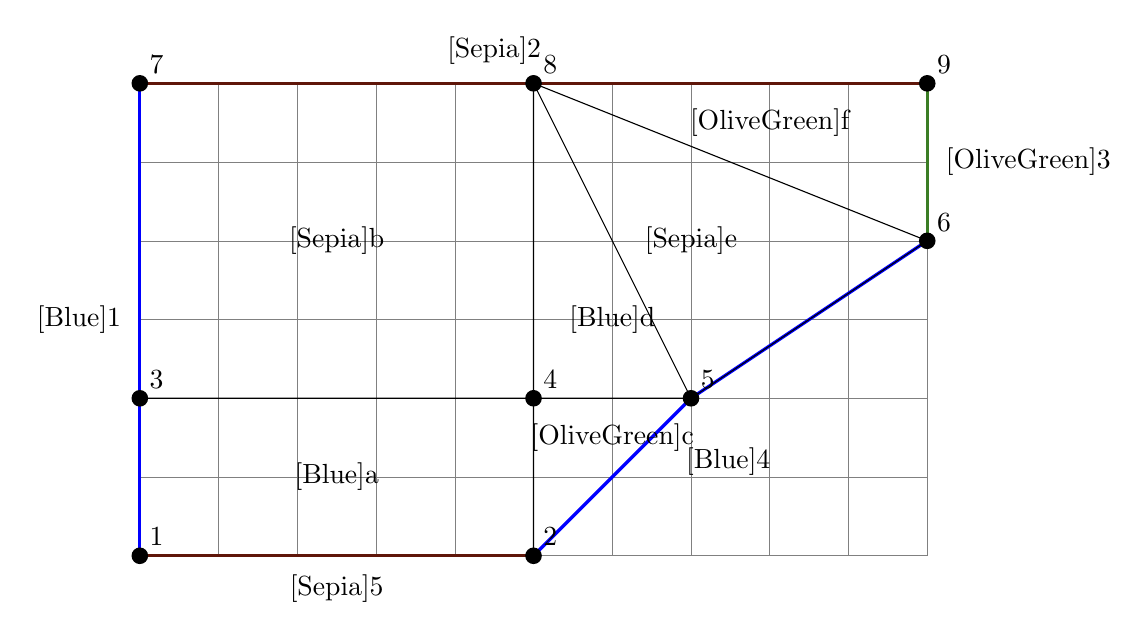
\begin{tikzpicture}[x=1cm,y=1cm]
  \newcommand{\bLab}[4][(0,0)]{
    % \node[fill=#2,text=white,#3] at #1 {#4};
    \node[#3] at #1 {
      \bLabBox[#2]{#4}
    };
  }

  \begin{scope}[very thick]
    \draw[style=help lines,step=1cm] (0,0) grid (10,6);
    % \tikzstyle{every node}=[draw,circle]

    \draw[draw=\mycola] (0,0) -- (0,6);
    \bLab[(0-0.1,3)]{\mycola}{left}{1}

    \draw[draw=\mycolb] (0,6) -- (10,6);
    \bLab[(4.5,6.1)]{\mycolb}{above}{2}

    \draw[draw=\mycolc] (10,6) -- (10,4);
    \bLab[(10.1,5)]{\mycolc}{right}{3}

    \draw[draw=\mycola] (10,4) -- (7,2) -- (5,0);
    \bLab[(7-0.2,1.2)]{\mycola}{right}{4}

    \draw[draw=\mycolb] (5,0) -- (0,0);
    \bLab[(2.5,-0.1)]{\mycolb}{below}{5}
  \end{scope}

  \begin{scope}
    % draw the mesh
    \draw (0,2) -- +(7,0)
    (5,0) -- ++(0,6)
     -- +(2,-4)
     -- +(5,-2)
     -- +(0,0);

     \foreach \x/\y/\l in {
       0/0/1,5/0/2,0/2/3,5/2/4,
       7/2/5,10/4/6,0/6/7,5/6/8,
       10/6/9}{
       \fill[black] (\x,\y) circle (3pt);
       \node[above right] at (\x,\y) {\l};
     }

     \newcommand{\nLab}[3][(0,0)]{
       % \node[fill=#2,text=white,rectangle] at #1 {#3};
       \node at #1 {\nLabBox[#2]{#3}};
     }

     \foreach \x/\y/\l/\c in {
       2.5/1/a/\mycola,2.5/4/b/\mycolb,
       6/1.5/c/\mycolc,6/3/d/\mycola,
       7/4/e/\mycolb,8/5.5/f/\mycolc
     }{\nLab[(\x,\y)]{\c}{\l}}
  \end{scope}
\end{tikzpicture}

\MySet{bd.col.1}{\mycola}
\MySet{bd.col.2}{\mycolb}
\MySet{bd.col.3}{\mycolc}
\MySet{bd.col.4}{\mycola}
\MySet{bd.col.5}{\mycolb}
\foreach \n/\i in {
  1/\mycola,
  2/\mycolb,
  3/\mycolc,
  4/\mycola,
  5/\mycolb}{
  \MySet{bd.col.\n}{\i}
}

\newcommand{\bd}[1]{\bLabBox[\MyGet{bd.col.#1}]{#1}}
\newcommand{\el}[1]{\nLabBox[\MyGet{el.col.#1}]{#1}}

% \foreach \n/\i in {
%   a/\mycola,
%   b/\mycolb,
%   c/\mycolc,
%   d/\mycola,
%   e/\mycolb,
%   f/\mycolc}{
%   \MySet{el.col.\n}{\i}
% }
% Don't know why it dosn't work   
\MySet{el.col.a}{\mycola}
\MySet{el.col.b}{\mycolb}
\MySet{el.col.c}{\mycolc}
\MySet{el.col.d}{\mycola}
\MySet{el.col.e}{\mycolb}
\MySet{el.col.f}{\mycolc}

Where \bd{1} to \bd{5} are boundaries,
and \el{a} to \el{f} are elements.

And the BCs are:
\def\f#1{\mbox{Along \bd{#1}: }}
\begin{align}
    \f{1} & \phin = 0 &  \f{2} & \phi = au_0 \notag\\
    \f{3} & \phin = 0 & \f{4} & \phi = 0 \notag\\ 
    \f{5} & \phi = 0 && \notag
\end{align}
\end{questionbox}

\subsection*{Answer}\label{sec:q2}
\subsubsection*{Weak formulation}
Let $v$ be an arbitrary test function, the weak formulation of \cref{eq:poi} is
then
\newcommand{\inta}[1]{
  \ensuremath{\int_{\text{Domain}} #1 \text{dA}}
}
\newcommand{\intb}[1]{
  \ensuremath{\int_{\text{Boundary}} #1 \text{ds}}
}

\def\x{
  \ensuremath{\inta{\nabla \phi \bullet \nabla v}}
}
\def\y{
  \ensuremath{\intb{\phin v}}
}


\begin{align}
  0 &= \inta{(\dxx{\phi} + \dyy{\phi}) v} \notag\\
  \intertext{By Gauss-Green}
    &= \inta{-\dx{\phi}\dx{v} - \dy{\phi}\dy{v}} +
      \intb{
      (\dx{\phi}\dx{n} + \dy{\phi}\dy{n})v
      } \notag\\
    &= -\x + \y \notag
\end{align}
Therefore,
\begin{align}
  \x &= \y \label{eq:tosub}
\end{align}
Now according to Galerkin's method, we take $v = \phi = N_j\phi_j$, which gives
\begin{align}
  \nabla v &= \nabla \phi = \nabla (N_i \phi_i) \notag\\
           &= \sum_i \phi_i \nabla N_i \notag\\
  &= \sum_i \phi_i
    \begin{bmatrix}
      \dx{N_i} \\ \dy{N_i}
    \end{bmatrix} \notag
\end{align}
Therefore, substituting the above into \cref{eq:tosub} gives
\def\x{\ensuremath{\inta{\nabla (N_i)\nabla (N_j)}}}
\def\bi{\ensuremath{\intb{\phin N_i}}}
\begin{align}
  \phi_i \inta{\nabla N_i \nabla N_j} \phi_j &= \intb{\phin N_j \phi_j} \notag\\
  \phi_i K_{ij} \phi_j &= b_i \phi_i \notag\\
  \intertext{Where}
  K_{ij} &= \x = \inta{\dx{N_i}\dx{N_j} + \dy{N_x}\dy{N_j}} \notag\\
  b_i &= \bi \notag
\end{align}
Taking derivatives with respect to $\mathbf{\phi} = [\phi_1, \dotsc, \phi_n]$,
and setting it to 0 gives the finite element equation
\def\tr#1{\ensuremath{{#1}^{\text{T}}}}
\def\p{\mathbf{\phi}}
\begin{align}
  \dX[\p]{\tr{\p} \mathbf{K} \p - \tr{\p}\mathbf{b}} &= 0 \quad \Rightarrow \quad
                                                       \mathbf{K}\p = \mathbf{b}
                                                       \label{eq:fe} \\
  \intertext{Where}
  \mathbf{K}_{ij} &= K_{ij} \quad \mathbf{b}_{i} &= b_i \notag
\end{align}
\def\K{\ensuremath{\mathbf{K}}}
We calculate \K element by element. But before we start, we derive the general
formulae that calculate the ``local stiffness matrix'' $K_{ij} = \x $ on a
rectangular element and a triangular element.

\subsubsection*{Local stiffness matrix for a rectangular element}
For a rectangular element as shown below

\begin{center}
  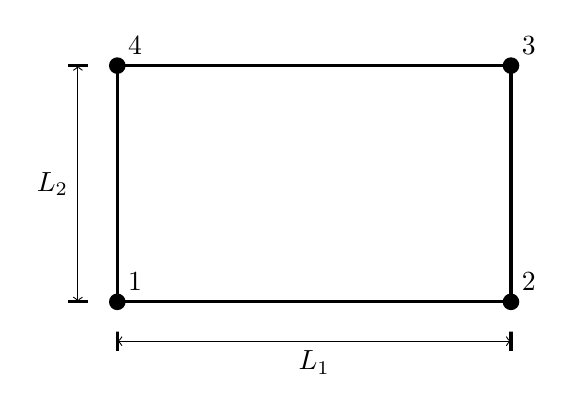
\begin{tikzpicture}[x=1cm,y=1cm]
  \begin{scope}[very thick]
    \draw (0,0) node[above right] (n1) {1}
    --  +(5,0) node[above right] (n2) {2}
    -- +(5,3) node[above right] (n3) {3}
    -- +(0,3) node[above right] (n4) {4}
    -- cycle;

    \foreach \i in {1,2,3,4}{
      % \node[fill=#2,]
      \fill[black] (n\i.south west) circle (3pt);
    }

    \newdimen\h
    \h=3.5pt
    % Draw the two dimensions
    \def\i{0.5cm}
    \def\j{5cm}

    \draw[thin,<->] (0,-\i) to node[anchor=north] {$L_1$} +(\j,0);
    \draw (0,-\i) -- +(0,\h) -- +(0, -\h)
    (\j,-\i) -- +(0,\h) -- +(0, -\h);

    % y dimensions
    \newcommand{\mydimy}[4]{%
      \draw[thin,<->] (#1,#2) to node[left] {#4} +(0,#3);
      \draw (#1,#2) -- +(-\h,0) -- +(\h,0)
      (#1,#2 + #3) --  +(-\h,0) -- +(\h,0);
    }
    \mydimy{-0.5cm}{0}{3}{$L_{2}$}
  \end{scope}
\end{tikzpicture}
\end{center}

\newcommand{\shpf}{shape functions}
The \shpf{} are
\newcommand{\Ni}[1]{\ensuremath{N_i(x,y)}}
\newcommand{\Nij}[2]{\dX[#2]{N_{#1}}}
\def\g#1{\ensuremath{g_{#1}(y)}}
\def\f#1{\ensuremath{f_{#1}(x)}}
\newcommand{\vg}{
  \begin{bmatrix}
    \g2 \\ \g1
  \end{bmatrix}
}

\begin{align}
  \begin{bmatrix}
    \Ni{4} & \Ni{3}\\
    \Ni{1} & \Ni{2}
  \end{bmatrix} &= \vg
             \begin{bmatrix}
               \f1 & \f2
             \end{bmatrix} \notag\\
  \intertext{Where}
  \begin{bmatrix}
    \f2\\ \f1
  \end{bmatrix}
           &=
             \begin{bmatrix}
               f_2\\f_1
             \end{bmatrix}
           =
                  \begin{bmatrix}
                    \frac{x}{L1} \\
                    1 - \f2
                  \end{bmatrix} \notag\\
  \vg &=
        \begin{bmatrix}
          g_2\\g_1
        \end{bmatrix}
           =
             \begin{bmatrix}
               \frac{y}{L2} \\
               1 - \g2
             \end{bmatrix} \notag
  \intertext{And their derivatives are}
  \begin{bmatrix}
    f_2' \\
    f_1'
  \end{bmatrix}
           &=
             \begin{bmatrix}
               \frac{1}{L1}\\
               - f_2'
             \end{bmatrix} \notag\\
  \begin{bmatrix}
    g_2' \\
    g_1'
  \end{bmatrix}
           &=
             \begin{bmatrix}
               \frac{1}{L2}\\
               - g_2'
             \end{bmatrix} \label{eq:fgvals}
\end{align}
Note that we have arranged the \shpf{} such that their position on the matrix above
are similar to their corresponding nodes on the figure above.

Now we calculate \Nij{i}{x} and \Nij{i}{y}
\newcommand{\Nx}{\ensuremath{\dx{\mathbf{N}}}}
\newcommand{\Ny}{\ensuremath{\dy{\mathbf{N}}}}

\def\mv#1#2{
  \ensuremath{\begin{bmatrix}#1 \\ #2\end{bmatrix}}
}
\def\mh#1#2{
  \ensuremath{\begin{bmatrix}#1 & #2\end{bmatrix}}
}
\def\x{\mv{g_2}{g_1}}
\def\y{
  % \ensuremath{\begin{bmatrix} f_1 & f_2 \end{bmatrix}}
  \ensuremath{\mh{f_1}{f_2}}
}
\begin{align}
  \Nx &=
        \begin{bmatrix}
          \Nij{4}{x} & \Nij{3}{x} \\
          \Nij{1}{x} & \Nij{2}{x} 
        \end{bmatrix}
                       = \x \mh{f_1'}{f_2'} = \x \mh{-f_2'}{f_2'}
                       = f_2' \x \mh{-1}{1}
                       \notag\\
  \Ny &=
        \begin{bmatrix}
          \Nij{4}{y} & \Nij{3}{y} \\
          \Nij{1}{y} & \Nij{2}{y} 
        \end{bmatrix}
                       = \mv{g_2'}{g_1'} \y = \mv{g_2'}{-g_2'} \y
                       = g_2'\mv{1}{-1} \y \notag
\end{align}
\def\Kx{\ensuremath{\mathbf{K_x}}}
\def\Ky{\ensuremath{\mathbf{K_y}}}
\newcommand{\Mij}[1]{
  \ensuremath{
    {\left[ #1 \right]}_{ij}
  }
}
Now er define two matrices \Kx and \Ky as follows:
\newcommand{\intc}[1]{
  \ensuremath{\int_0^{L2} \int_0^{L1} #1 \text{dxdy}}
}
\begin{align}
  \K &= \Kx + \Ky \notag\\
  \intertext{Where}
  \Mij{\Kx} &= \intc{\Nij{i}{x} \Nij{j}{x}} \notag\\
  \Mij{\Ky} &= \intc{\Nij{i}{y} \Nij{j}{y}} \notag
\end{align}
Next we flatten the (derivatives) \shpf{} matrices into column vectors by
defining:
\def\f#1{\ensuremath{N_{#1} &=
    \begin{bmatrix}
      \Nij{1}{#1} &
      \Nij{2}{#1} &
      \Nij{3}{#1} &
      \Nij{4}{#1} 
    \end{bmatrix}
  }
}
\begin{align}
  \f{x} \notag\\
  \f{y} \notag
\end{align}
So, $K_x$ and $K_y$ are
\begin{align}
  K_x &= \intc{\tr{N_x}N_x} \notag\\ 
  K_y &= \intc{\tr{N_y}N_y} \notag
\end{align}
Substituting the values in \cref{eq:fgvals} gives

\newcommand{\G}[1]{\MyGet{#1}}
\begin{align}
  K &= K_x + K_y \label{eq:recK} \\
  K_x &= \frac{1}{6} \frac{L_2}{L_1} \G{rec.Kx} \notag\\ 
  K_y &= \frac{1}{6} \frac{L_1}{L_2} \G{rec.Ky} \notag
\end{align}

\subsubsection*{Local stiffness matrix for a triangular element}
For a triangular element as shown below

\begin{center}
\begin{tikzpicture}[x=1cm,y=1cm]
  \begin{scope}
    \draw (0,0) coordinate (n1)
    --  +(4,-1) coordinate (n2) 
    -- +(3,2) coordinate (n3)
    -- cycle;

    \foreach \i/\p in {1/above left,2/below right,
      3/above left}{
      \node[\p] at (n\i) {$(x_{\i}, y_{\i})$};
      \fill[black] (n\i) circle (3pt);
    }
  \end{scope}
\end{tikzpicture}
\end{center}

The \shpf{} are
\def\N{\ensuremath{\mathbf{N}}}
\def\B{\ensuremath{\mathbf{B}}}
\def\A{\ensuremath{\mathbf{A}}}
\def\vxy{\ensuremath{\begin{bmatrix} 1&x&y \end{bmatrix}}}
\begin{align}
  \N &=
       \begin{bmatrix}
         \Ni{1} & \Ni{2} & \Ni{3} 
       \end{bmatrix} \notag\\
     &= \vxy \B = \vxy
       \begin{bmatrix} r_1 \\ r_2 \\ r_3 \end{bmatrix} \notag\\
  &= r_1 + xr_2 + yr_3
  \intertext{Where}
  r_i &= \text{The $i^{th}$ row of \B} \notag\\
  \B &= \A^{-1} \notag\\
  \A &=
       \begin{bmatrix}
         1 & x_1 & y_1 \\
         1 & x_2 & y_2 \\
         1 & x_3 & y_3 
       \end{bmatrix} \notag
\end{align}
Note that \shpf{} are linear, so their derivatives with respect to $x$ and $y$
are constant, which turns out to be entries in \B.
\def\f#1{
  \ensuremath{
    N_{#1} := \dX[#1]{\N} =
    \tr{
      \begin{bmatrix}
        \dX[#1]{N_1} &
        \dX[#1]{N_2} &
        \dX[#1]{N_3} 
      \end{bmatrix}
    }
      }
    }
\begin{align}
  \f{x} = r_2 \notag\\
  \f{y} = r_3 \notag
\end{align}
Similar to what we have done to for the rectanglar element, we define \Kx and
\Ky as follows:

\newcommand{\intd}[1]{
  \ensuremath{
    \int_{\text{A}}
    #1
    \text{dA}
  }
}
\def\f#1{
  \ensuremath{
    \Mij{K_{#1}} := \intd{\dX[#1]{N_i} \dX[#1]{N_j}}
  }
}
\def\dN#1{
  \ensuremath{\dX[#1]{\N}}
}
\def\dNdN#1{\tr{N_{x}}N_{x}}

\begin{align}
  \f{x} \notag\\
  \f{y}
  \notag
\end{align}
Where integrate over A means ``Integrate over the entire triangular element''.
However, since $N_x$ and $N_y$ are actually constant vector, therefore
\def\ar{ \text{area of triangular element}}
\begin{align}
  K_x  = \intd{\dNdN{x}} = r_2\tr{r_2} \intd{} = \ar \notag\\ 
  K_y = \intd{\dNdN{y}}  = r_2\tr{r_3} \intd{} = \ar \notag\\
  \intertext{So}
  \K = [r_2\tr{r_2} + r_3\tr{r_3}] \times \ar \label{eq:triK}
\end{align}

\subsubsection*{Calculate \K element by element}
\newcommand{\globalK}[1]{
  And its contribution to global stiffness matrix is
\begin{align}
  K_{#1,\text{global}} = \G{K.g.#1} \label{eq:K.g.#1}
\end{align}
}
\newcommand{\rec}[1]{%
  \paragraph{For element #1} applying \cref{eq:recK}
  with $L_1 =
  \G{l1.#1}, L_2 = \G{l2.#1}$ gives
\begin{align}
  K_{x,#1} &= \G{Kx.#1} \notag\\
  K_{y,#1} &= \G{Ky.#1} \notag\\
  K_{#1} &= \G{K.#1} \notag
\end{align}
\globalK{#1}
}
\newcommand{\tri}[1]{
  \paragraph{For element #1} applying \cref{eq:triK} with
  \begin{align*}
    \A = \begin{bmatrix}
      1 & x_1 & y_1 \\
      1 & x_2 & y_2 \\
      1 & x_3 & y_3 
    \end{bmatrix} = \G{A.#1}
  \end{align*} gives
  \begin{align}
    \B &= \A^{-1} = \G{B.#1} \notag\\
    \K &= \left[
         \G{B.r2.#1} \G{B.r2.t.#1}
         +
         \G{B.r3.#1} \G{B.r3.t.#1}
         \right]
         \G{Area.#1} \notag
\end{align}
\globalK{#1}
}
\rec{a}
\rec{b}
\tri{c}
\tri{d}
\tri{e}
\tri{f}
Now summing up \cref{eq:K.g.a,eq:K.g.b,eq:K.g.c,eq:K.g.d,eq:K.g.e,eq:K.g.f}
gives the global stiffness matrix \K
\begin{align}
  K_{\text{global}} &=
                      K_{a,\text{global}}
                      \foreach \i in {b,c,d,e,f}{
                      + 
                      K_{\i,\text{global}}
                      }\notag\\ 
  &= \G{K.g}
\end{align}

To finish \cref{eq:fe}, we apply the BCs, which can be more or less translated
into the following:
\def\DOF{degree of freedom}
\begin{quote}
  On all nodes except for node 3 and 4,
  the values of $\phi$ are known (so  \DOF{}$-7$). However, for each of these
  node (7 nodes), a nonzero value of $b_i = \bi$ is added for them.
\end{quote}
So
\def\au{\ensuremath{au_0}}
\begin{align}
  \mathbf{b} &=
               \tr{\begin{bmatrix}
                 b_1 & b_2 & 0&0&b_5&b_6&b_7&b_8&b_9
               \end{bmatrix}}
                                                  \notag\\
  \intertext{And}
  \mathbf{\phi}
             &=
                  \tr{\begin{bmatrix}
                      b_1 & b_2 & 0&0&b_5&b_6&b_7&b_8&b_9
                    \end{bmatrix}} \notag\\
             &=
               \tr{\begin{bmatrix}
                   \phi_1 , \dotsc \phi_9
                 \end{bmatrix}} \notag\\
             &=
               \tr{\begin{bmatrix}
                   0&0&\phi_3&\phi_4&0&0&\au&\au&\au
                 \end{bmatrix}}
\end{align}
So the system is therefore
\def\bn{\ensuremath{
    \begin{bmatrix}
      b_1 \\ b_2 \\ 0 \\ 0 \\ b_5 \\ b_6 \\ b_7 \\ b_8 \\ b_9 
    \end{bmatrix}}}
\def\phin{\ensuremath{
    \begin{bmatrix}
      0\\0\\\phi_3\\\phi_4\\0\\0\\ \au \\ \au \\ \au
    \end{bmatrix}}}
\begin{align*}
  \K \mathbf{\phi} = \mathbf{b} \notag\\
  \G{K.g} \phin = \bn \notag
\end{align*}
We first solve for $\phi_2$ and $\phi_3$
\def\one{\ensuremath{
    \begin{bmatrix} 1\\1\\1
    \end{bmatrix}}}
\def\pp{\ensuremath{
    \begin{bmatrix} \phi_3 \\ \phi_4
    \end{bmatrix}}}
\begin{align}
  \G{K.g.sm} \phin &= \bn \notag\\
  \G{K.g.m1} \pp &= - \G{K.g.m2} \one \au \notag\\
  \G{K.g.m1}^{-1} \pp &= \G{K.g.mi.inv} \notag\\
  -\au \G{K.g.m2} \one &= \au \G{K.g.m3} \notag\\
  \pp &= \au \begin{bmatrix} \G{phi3}\\\G{phi4} \end{bmatrix} \notag
\end{align}

And now $\mathbf{b}$ can be calculated as
\begin{align}
  \mathbf{b} = \au \G{K.g}
  \begin{bmatrix}
    0\\0\\\G{phi3}\\\G{phi4}\\0\\0\\ \au \\ \au \\ \au
  \end{bmatrix}
  = \au \G{b.n}
\end{align}

\subsubsection*{Remarks}
And the contour is shown below

% Created by tikzDevice version 0.12.3.1 on 2022-03-13 23:33:43
% !TEX encoding = UTF-8 Unicode
\begin{tikzpicture}[x=1pt,y=1pt]
\definecolor{fillColor}{RGB}{255,255,255}
\path[use as bounding box,fill=fillColor,fill opacity=0.00] (0,0) rectangle (867.24,361.35);
\begin{scope}
\path[clip] (  0.00,  0.00) rectangle (867.24,361.35);
\definecolor{drawColor}{RGB}{255,255,255}
\definecolor{fillColor}{RGB}{255,255,255}

\path[draw=drawColor,line width= 0.6pt,line join=round,line cap=round,fill=fillColor] (  0.00,  0.00) rectangle (867.24,361.35);
\end{scope}
\begin{scope}
\path[clip] ( 14.85, 18.22) rectangle (804.15,355.85);
\definecolor{fillColor}{gray}{0.92}

\path[fill=fillColor] ( 14.85, 18.22) rectangle (804.15,355.85);
\definecolor{drawColor}{RGB}{255,255,255}

\path[draw=drawColor,line width= 0.3pt,line join=round] ( 14.85, 42.09) --
	(804.15, 42.09);

\path[draw=drawColor,line width= 0.3pt,line join=round] ( 14.85,161.46) --
	(804.15,161.46);

\path[draw=drawColor,line width= 0.3pt,line join=round] ( 14.85,280.82) --
	(804.15,280.82);

\path[draw=drawColor,line width= 0.3pt,line join=round] (140.42, 18.22) --
	(140.42,355.85);

\path[draw=drawColor,line width= 0.3pt,line join=round] (319.80, 18.22) --
	(319.80,355.85);

\path[draw=drawColor,line width= 0.3pt,line join=round] (499.19, 18.22) --
	(499.19,355.85);

\path[draw=drawColor,line width= 0.3pt,line join=round] (678.58, 18.22) --
	(678.58,355.85);

\path[draw=drawColor,line width= 0.6pt,line join=round] ( 14.85,101.78) --
	(804.15,101.78);

\path[draw=drawColor,line width= 0.6pt,line join=round] ( 14.85,221.14) --
	(804.15,221.14);

\path[draw=drawColor,line width= 0.6pt,line join=round] ( 14.85,340.50) --
	(804.15,340.50);

\path[draw=drawColor,line width= 0.6pt,line join=round] ( 50.73, 18.22) --
	( 50.73,355.85);

\path[draw=drawColor,line width= 0.6pt,line join=round] (230.11, 18.22) --
	(230.11,355.85);

\path[draw=drawColor,line width= 0.6pt,line join=round] (409.50, 18.22) --
	(409.50,355.85);

\path[draw=drawColor,line width= 0.6pt,line join=round] (588.88, 18.22) --
	(588.88,355.85);

\path[draw=drawColor,line width= 0.6pt,line join=round] (768.27, 18.22) --
	(768.27,355.85);
\definecolor{drawColor}{RGB}{35,75,110}
\definecolor{fillColor}{RGB}{35,75,110}

\path[draw=drawColor,line width= 0.4pt,line join=round,line cap=round,fill=fillColor] ( 50.73, 33.57) circle (  1.96);
\definecolor{drawColor}{RGB}{36,77,113}
\definecolor{fillColor}{RGB}{36,77,113}

\path[draw=drawColor,line width= 0.4pt,line join=round,line cap=round,fill=fillColor] (153.23, 33.57) circle (  1.96);
\definecolor{drawColor}{RGB}{38,80,117}
\definecolor{fillColor}{RGB}{38,80,117}

\path[draw=drawColor,line width= 0.4pt,line join=round,line cap=round,fill=fillColor] (255.74, 33.57) circle (  1.96);
\definecolor{drawColor}{RGB}{39,82,120}
\definecolor{fillColor}{RGB}{39,82,120}

\path[draw=drawColor,line width= 0.4pt,line join=round,line cap=round,fill=fillColor] (358.24, 33.57) circle (  1.96);
\definecolor{drawColor}{RGB}{30,64,95}
\definecolor{fillColor}{RGB}{30,64,95}

\path[draw=drawColor,line width= 0.4pt,line join=round,line cap=round,fill=fillColor] (460.75, 33.57) circle (  1.96);
\definecolor{drawColor}{RGB}{30,65,97}
\definecolor{fillColor}{RGB}{30,65,97}

\path[draw=drawColor,line width= 0.4pt,line join=round,line cap=round,fill=fillColor] ( 50.73, 84.72) circle (  1.96);
\definecolor{drawColor}{RGB}{31,66,98}
\definecolor{fillColor}{RGB}{31,66,98}

\path[draw=drawColor,line width= 0.4pt,line join=round,line cap=round,fill=fillColor] (153.23, 84.72) circle (  1.96);
\definecolor{drawColor}{RGB}{31,67,99}
\definecolor{fillColor}{RGB}{31,67,99}

\path[draw=drawColor,line width= 0.4pt,line join=round,line cap=round,fill=fillColor] (255.74, 84.72) circle (  1.96);
\definecolor{drawColor}{RGB}{31,67,100}
\definecolor{fillColor}{RGB}{31,67,100}

\path[draw=drawColor,line width= 0.4pt,line join=round,line cap=round,fill=fillColor] (358.24, 84.72) circle (  1.96);
\definecolor{drawColor}{RGB}{34,73,108}
\definecolor{fillColor}{RGB}{34,73,108}

\path[draw=drawColor,line width= 0.4pt,line join=round,line cap=round,fill=fillColor] (460.75, 84.72) circle (  1.96);
\definecolor{drawColor}{RGB}{56,116,165}
\definecolor{fillColor}{RGB}{56,116,165}

\path[draw=drawColor,line width= 0.4pt,line join=round,line cap=round,fill=fillColor] ( 50.73,135.88) circle (  1.96);
\definecolor{drawColor}{RGB}{57,119,169}
\definecolor{fillColor}{RGB}{57,119,169}

\path[draw=drawColor,line width= 0.4pt,line join=round,line cap=round,fill=fillColor] (153.23,135.88) circle (  1.96);
\definecolor{drawColor}{RGB}{59,122,173}
\definecolor{fillColor}{RGB}{59,122,173}

\path[draw=drawColor,line width= 0.4pt,line join=round,line cap=round,fill=fillColor] (255.74,135.88) circle (  1.96);
\definecolor{drawColor}{RGB}{60,125,178}
\definecolor{fillColor}{RGB}{60,125,178}

\path[draw=drawColor,line width= 0.4pt,line join=round,line cap=round,fill=fillColor] (358.24,135.88) circle (  1.96);
\definecolor{drawColor}{RGB}{42,89,128}
\definecolor{fillColor}{RGB}{42,89,128}

\path[draw=drawColor,line width= 0.4pt,line join=round,line cap=round,fill=fillColor] (460.75,135.88) circle (  1.96);
\definecolor{drawColor}{RGB}{34,72,106}
\definecolor{fillColor}{RGB}{34,72,106}

\path[draw=drawColor,line width= 0.4pt,line join=round,line cap=round,fill=fillColor] (563.26,135.88) circle (  1.96);
\definecolor{drawColor}{RGB}{46,97,139}
\definecolor{fillColor}{RGB}{46,97,139}

\path[draw=drawColor,line width= 0.4pt,line join=round,line cap=round,fill=fillColor] ( 50.73,187.04) circle (  1.96);
\definecolor{drawColor}{RGB}{48,101,145}
\definecolor{fillColor}{RGB}{48,101,145}

\path[draw=drawColor,line width= 0.4pt,line join=round,line cap=round,fill=fillColor] (153.23,187.04) circle (  1.96);
\definecolor{drawColor}{RGB}{50,105,150}
\definecolor{fillColor}{RGB}{50,105,150}

\path[draw=drawColor,line width= 0.4pt,line join=round,line cap=round,fill=fillColor] (255.74,187.04) circle (  1.96);
\definecolor{drawColor}{RGB}{52,109,155}
\definecolor{fillColor}{RGB}{52,109,155}

\path[draw=drawColor,line width= 0.4pt,line join=round,line cap=round,fill=fillColor] (358.24,187.04) circle (  1.96);
\definecolor{drawColor}{RGB}{51,108,154}
\definecolor{fillColor}{RGB}{51,108,154}

\path[draw=drawColor,line width= 0.4pt,line join=round,line cap=round,fill=fillColor] (460.75,187.04) circle (  1.96);
\definecolor{drawColor}{RGB}{42,89,129}
\definecolor{fillColor}{RGB}{42,89,129}

\path[draw=drawColor,line width= 0.4pt,line join=round,line cap=round,fill=fillColor] (563.26,187.04) circle (  1.96);
\definecolor{drawColor}{RGB}{33,70,103}
\definecolor{fillColor}{RGB}{33,70,103}

\path[draw=drawColor,line width= 0.4pt,line join=round,line cap=round,fill=fillColor] (665.76,187.04) circle (  1.96);
\definecolor{drawColor}{RGB}{37,78,114}
\definecolor{fillColor}{RGB}{37,78,114}

\path[draw=drawColor,line width= 0.4pt,line join=round,line cap=round,fill=fillColor] ( 50.73,238.19) circle (  1.96);
\definecolor{drawColor}{RGB}{39,83,121}
\definecolor{fillColor}{RGB}{39,83,121}

\path[draw=drawColor,line width= 0.4pt,line join=round,line cap=round,fill=fillColor] (153.23,238.19) circle (  1.96);
\definecolor{drawColor}{RGB}{42,88,127}
\definecolor{fillColor}{RGB}{42,88,127}

\path[draw=drawColor,line width= 0.4pt,line join=round,line cap=round,fill=fillColor] (255.74,238.19) circle (  1.96);
\definecolor{drawColor}{RGB}{44,93,134}
\definecolor{fillColor}{RGB}{44,93,134}

\path[draw=drawColor,line width= 0.4pt,line join=round,line cap=round,fill=fillColor] (358.24,238.19) circle (  1.96);
\definecolor{drawColor}{RGB}{61,127,180}
\definecolor{fillColor}{RGB}{61,127,180}

\path[draw=drawColor,line width= 0.4pt,line join=round,line cap=round,fill=fillColor] (460.75,238.19) circle (  1.96);
\definecolor{drawColor}{RGB}{51,107,153}
\definecolor{fillColor}{RGB}{51,107,153}

\path[draw=drawColor,line width= 0.4pt,line join=round,line cap=round,fill=fillColor] (563.26,238.19) circle (  1.96);
\definecolor{drawColor}{RGB}{41,87,126}
\definecolor{fillColor}{RGB}{41,87,126}

\path[draw=drawColor,line width= 0.4pt,line join=round,line cap=round,fill=fillColor] (665.76,238.19) circle (  1.96);
\definecolor{drawColor}{RGB}{36,77,113}
\definecolor{fillColor}{RGB}{36,77,113}

\path[draw=drawColor,line width= 0.4pt,line join=round,line cap=round,fill=fillColor] (768.27,238.19) circle (  1.96);
\definecolor{drawColor}{RGB}{28,60,90}
\definecolor{fillColor}{RGB}{28,60,90}

\path[draw=drawColor,line width= 0.4pt,line join=round,line cap=round,fill=fillColor] ( 50.73,289.35) circle (  1.96);
\definecolor{drawColor}{RGB}{30,66,98}
\definecolor{fillColor}{RGB}{30,66,98}

\path[draw=drawColor,line width= 0.4pt,line join=round,line cap=round,fill=fillColor] (153.23,289.35) circle (  1.96);
\definecolor{drawColor}{RGB}{33,71,105}
\definecolor{fillColor}{RGB}{33,71,105}

\path[draw=drawColor,line width= 0.4pt,line join=round,line cap=round,fill=fillColor] (255.74,289.35) circle (  1.96);
\definecolor{drawColor}{RGB}{36,77,113}
\definecolor{fillColor}{RGB}{36,77,113}

\path[draw=drawColor,line width= 0.4pt,line join=round,line cap=round,fill=fillColor] (358.24,289.35) circle (  1.96);
\definecolor{drawColor}{RGB}{71,147,206}
\definecolor{fillColor}{RGB}{71,147,206}

\path[draw=drawColor,line width= 0.4pt,line join=round,line cap=round,fill=fillColor] (460.75,289.35) circle (  1.96);
\definecolor{drawColor}{RGB}{60,125,178}
\definecolor{fillColor}{RGB}{60,125,178}

\path[draw=drawColor,line width= 0.4pt,line join=round,line cap=round,fill=fillColor] (563.26,289.35) circle (  1.96);

\path[draw=drawColor,line width= 0.4pt,line join=round,line cap=round,fill=fillColor] (665.76,289.35) circle (  1.96);

\path[draw=drawColor,line width= 0.4pt,line join=round,line cap=round,fill=fillColor] (768.27,289.35) circle (  1.96);
\definecolor{drawColor}{RGB}{19,43,67}
\definecolor{fillColor}{RGB}{19,43,67}

\path[draw=drawColor,line width= 0.4pt,line join=round,line cap=round,fill=fillColor] ( 50.73,340.50) circle (  1.96);
\definecolor{drawColor}{RGB}{22,49,75}
\definecolor{fillColor}{RGB}{22,49,75}

\path[draw=drawColor,line width= 0.4pt,line join=round,line cap=round,fill=fillColor] (153.23,340.50) circle (  1.96);
\definecolor{drawColor}{RGB}{25,56,84}
\definecolor{fillColor}{RGB}{25,56,84}

\path[draw=drawColor,line width= 0.4pt,line join=round,line cap=round,fill=fillColor] (255.74,340.50) circle (  1.96);
\definecolor{drawColor}{RGB}{29,62,93}
\definecolor{fillColor}{RGB}{29,62,93}

\path[draw=drawColor,line width= 0.4pt,line join=round,line cap=round,fill=fillColor] (358.24,340.50) circle (  1.96);
\definecolor{drawColor}{RGB}{86,177,247}
\definecolor{fillColor}{RGB}{86,177,247}

\path[draw=drawColor,line width= 0.4pt,line join=round,line cap=round,fill=fillColor] (460.75,340.50) circle (  1.96);

\path[draw=drawColor,line width= 0.4pt,line join=round,line cap=round,fill=fillColor] (563.26,340.50) circle (  1.96);

\path[draw=drawColor,line width= 0.4pt,line join=round,line cap=round,fill=fillColor] (665.76,340.50) circle (  1.96);

\path[draw=drawColor,line width= 0.4pt,line join=round,line cap=round,fill=fillColor] (768.27,340.50) circle (  1.96);
\end{scope}
\begin{scope}
\path[clip] (  0.00,  0.00) rectangle (867.24,361.35);
\definecolor{drawColor}{gray}{0.30}

\node[text=drawColor,anchor=base east,inner sep=0pt, outer sep=0pt, scale=  0.88] at (  9.90, 98.75) {2};

\node[text=drawColor,anchor=base east,inner sep=0pt, outer sep=0pt, scale=  0.88] at (  9.90,218.11) {4};

\node[text=drawColor,anchor=base east,inner sep=0pt, outer sep=0pt, scale=  0.88] at (  9.90,337.47) {6};
\end{scope}
\begin{scope}
\path[clip] (  0.00,  0.00) rectangle (867.24,361.35);
\definecolor{drawColor}{gray}{0.20}

\path[draw=drawColor,line width= 0.6pt,line join=round] ( 12.10,101.78) --
	( 14.85,101.78);

\path[draw=drawColor,line width= 0.6pt,line join=round] ( 12.10,221.14) --
	( 14.85,221.14);

\path[draw=drawColor,line width= 0.6pt,line join=round] ( 12.10,340.50) --
	( 14.85,340.50);
\end{scope}
\begin{scope}
\path[clip] (  0.00,  0.00) rectangle (867.24,361.35);
\definecolor{drawColor}{gray}{0.20}

\path[draw=drawColor,line width= 0.6pt,line join=round] ( 50.73, 15.47) --
	( 50.73, 18.22);

\path[draw=drawColor,line width= 0.6pt,line join=round] (230.11, 15.47) --
	(230.11, 18.22);

\path[draw=drawColor,line width= 0.6pt,line join=round] (409.50, 15.47) --
	(409.50, 18.22);

\path[draw=drawColor,line width= 0.6pt,line join=round] (588.88, 15.47) --
	(588.88, 18.22);

\path[draw=drawColor,line width= 0.6pt,line join=round] (768.27, 15.47) --
	(768.27, 18.22);
\end{scope}
\begin{scope}
\path[clip] (  0.00,  0.00) rectangle (867.24,361.35);
\definecolor{drawColor}{gray}{0.30}

\node[text=drawColor,anchor=base,inner sep=0pt, outer sep=0pt, scale=  0.88] at ( 50.73,  7.21) {0.0};

\node[text=drawColor,anchor=base,inner sep=0pt, outer sep=0pt, scale=  0.88] at (230.11,  7.21) {2.5};

\node[text=drawColor,anchor=base,inner sep=0pt, outer sep=0pt, scale=  0.88] at (409.50,  7.21) {5.0};

\node[text=drawColor,anchor=base,inner sep=0pt, outer sep=0pt, scale=  0.88] at (588.88,  7.21) {7.5};

\node[text=drawColor,anchor=base,inner sep=0pt, outer sep=0pt, scale=  0.88] at (768.27,  7.21) {10.0};
\end{scope}
\begin{scope}
\path[clip] (  0.00,  0.00) rectangle (867.24,361.35);
\definecolor{fillColor}{RGB}{255,255,255}

\path[fill=fillColor] (815.15,137.79) rectangle (861.74,236.28);
\end{scope}
\begin{scope}
\path[clip] (  0.00,  0.00) rectangle (867.24,361.35);
\node[inner sep=0pt,outer sep=0pt,anchor=south west,rotate=  0.00] at (820.65, 143.29) {
	\pgfimage[width= 14.45pt,height= 72.27pt,interpolate=true]{p_ras1}};
\end{scope}
\begin{scope}
\path[clip] (  0.00,  0.00) rectangle (867.24,361.35);
\definecolor{drawColor}{RGB}{0,0,0}

\node[text=drawColor,anchor=base west,inner sep=0pt, outer sep=0pt, scale=  0.88] at (840.60,152.08) {0.00};

\node[text=drawColor,anchor=base west,inner sep=0pt, outer sep=0pt, scale=  0.88] at (840.60,167.16) {0.25};

\node[text=drawColor,anchor=base west,inner sep=0pt, outer sep=0pt, scale=  0.88] at (840.60,182.25) {0.50};

\node[text=drawColor,anchor=base west,inner sep=0pt, outer sep=0pt, scale=  0.88] at (840.60,197.33) {0.75};

\node[text=drawColor,anchor=base west,inner sep=0pt, outer sep=0pt, scale=  0.88] at (840.60,212.41) {1.00};
\end{scope}
\begin{scope}
\path[clip] (  0.00,  0.00) rectangle (867.24,361.35);
\definecolor{drawColor}{RGB}{0,0,0}

\node[text=drawColor,anchor=base west,inner sep=0pt, outer sep=0pt, scale=  1.10] at (820.65,222.13) {$\phi$};
\end{scope}
\begin{scope}
\path[clip] (  0.00,  0.00) rectangle (867.24,361.35);
\definecolor{drawColor}{RGB}{255,255,255}

\path[draw=drawColor,line width= 0.2pt,line join=round] (820.65,155.11) -- (823.54,155.11);

\path[draw=drawColor,line width= 0.2pt,line join=round] (820.65,170.19) -- (823.54,170.19);

\path[draw=drawColor,line width= 0.2pt,line join=round] (820.65,185.28) -- (823.54,185.28);

\path[draw=drawColor,line width= 0.2pt,line join=round] (820.65,200.36) -- (823.54,200.36);

\path[draw=drawColor,line width= 0.2pt,line join=round] (820.65,215.44) -- (823.54,215.44);

\path[draw=drawColor,line width= 0.2pt,line join=round] (832.21,155.11) -- (835.10,155.11);

\path[draw=drawColor,line width= 0.2pt,line join=round] (832.21,170.19) -- (835.10,170.19);

\path[draw=drawColor,line width= 0.2pt,line join=round] (832.21,185.28) -- (835.10,185.28);

\path[draw=drawColor,line width= 0.2pt,line join=round] (832.21,200.36) -- (835.10,200.36);

\path[draw=drawColor,line width= 0.2pt,line join=round] (832.21,215.44) -- (835.10,215.44);
\end{scope}
\end{tikzpicture}


We see that the value of $\phi$ gradually increase from bottom ($\phi=0$) to
top ($\phi=1$). More elements shall be used for an increased accuracy.




\end{document}